\documentclass[a4paper,11pt]{report}

\usepackage[utf8]{inputenc}
\usepackage[T1]{fontenc}
\usepackage[italian]{babel}
\usepackage{geometry}
\usepackage{hyperref}
\usepackage{graphicx}
\usepackage{tabularx}
\usepackage{array}
\usepackage{enumitem}
\usepackage{booktabs}
\usepackage{float}

\geometry{margin=2.5cm}
\setlength{\parskip}{0.5em}
\setlength{\parindent}{0pt}

\title{DietiEstates25\\\large Documentazione}
\author{%
  Progetto ING-SW -- DietiEstates25\\[0.5em]
  \small Università degli Studi di Napoli Federico II
}
\date{\today}

\begin{document}

\maketitle
\tableofcontents

\chapter{Documento dei Requisiti Software}

\section{Contesto e obiettivi}

DietiEstates25 è una piattaforma web per la gestione di servizi immobiliari multi-agenzia.\\
L'obiettivo principale del sistema è:

\begin{itemize}[nosep]
  \item \textbf{Centralizzare} la gestione di agenzie, agenti, immobili e clienti.
  \item \textbf{Permettere agli utenti finali} di cercare immobili (vendita/affitto) con ricerca avanzata e mappa interattiva.
  \item \textbf{Supportare gli attori professionali} (agenzie, agenti) nella pubblicazione e gestione degli immobili.
  \item \textbf{Garantire sicurezza} delle credenziali e una \emph{user experience} moderna, intuitiva e responsiva.
\end{itemize}

Lo stato attuale dell’implementazione copre:

\begin{itemize}[nosep]
  \item Autenticazione e registrazione (utente, agenzia, agenti).
  \item Gestione agenzie e agenti (creazione agenti da parte del manager dell’agenzia).
  \item Gestione immobili (creazione annuncio con dettagli completi, coordinate geografiche, foto, servizi).
  \item Ricerca avanzata con filtro su parametri multipli e supporto ricerca geografica per raggio.
  \item Profili agenti con biografia, foto, proprietà collegate e recensioni clienti.
  \item Gestione profilo utente (dati personali, password, foto profilo per agenti).
  \item Recensioni agenti (rating numerico + commento testuale).
  \item Login/registrazione con provider esterni (Google, Facebook, GitHub).
\end{itemize}

Funzionalità previste dal capitolato ma \textbf{non ancora implementate} (o pianificate come estensione futura):

\begin{itemize}[nosep]
  \item Prenotazione visite agli immobili con agenda condivisa.
  \item Gestione di offerte di acquisto/affitto (workflow proposta/controproposta).
  \item Tipologie dedicate per affitti brevi / case vacanze.
\end{itemize}

\section{Glossario}

\begin{table}[H]
\centering
\renewcommand{\arraystretch}{1.2}
\begin{tabularx}{\textwidth}{>{\bfseries}l X}
\toprule
Termine & Definizione \\
\midrule
Agenzia & Organizzazione immobiliare che utilizza la piattaforma. Modellata come entità \texttt{Agency} nel back-end.\\
Manager di agenzia & Utente che rappresenta il gestore dell’agenzia; registra l’agenzia e crea gli account degli agenti.\\
Agente & Professionista immobiliare associato ad una Agenzia, modellato come sottoclasse \texttt{Agent} di \texttt{User}.\\
Utente (cliente) & Utente registrato interessato alla ricerca di immobili (acquisto/affitto), con ruolo \texttt{USER}.\\
Account esterno & Account OAuth2 (Google, Facebook, GitHub) collegato all’utente; indicato dal campo \texttt{authProvider}.\\
Immobile / Property & Entità \texttt{Property}: rappresenta un annuncio immobiliare (titolo, descrizione, prezzo, parametri fisici, ecc.).\\
Annuncio & Sinonimo operativo di ``Immobile pubblicato'' sulla piattaforma.\\
Amenity / Servizio & Servizio/comfort associato a un immobile (\texttt{Amenity}: es. Wi-Fi, portineria, climatizzazione, garage).\\
Classe energetica & Indicatore di efficienza energetica (\texttt{EnergyClass}), memorizzato come enum.\\
Recensione & Valutazione di un agente da parte di un utente, con punteggio numerico e commento (\texttt{Review}).\\
Profilo agente & Vista pubblica con dati dell’agente: biografia, foto, recapiti, lista immobili, recensioni.\\
Profilo utente & Vista privata dove l’utente modifica nome, cognome, e-mail, password e (per agenti) foto/biografia.\\
Ricerca avanzata & Funzionalità di filtraggio immobili per parametri multipli (prezzo, stanze, città, classe energetica, ecc.).\\
Ricerca geografica & Ricerca immobili entro un raggio da un punto selezionato su mappa (latitudine/longitudine + raggio).\\
JWT & JSON Web Token usato per autenticazione stateless tra front-end Angular e API Spring Boot.\\
H2 & Database in-memory usato in sviluppo, configurato in modalità PostgreSQL.\\
S3 Storage & Sistema di storage (AWS S3) per file/foto, incapsulato in \texttt{StorageService}.\\
\bottomrule
\end{tabularx}
\caption{Glossario dei principali termini di dominio}
\end{table}

\section{Personas}

\subsection{Persona 1 -- Giulia}
\begin{figure}[H]
    \centering
    
\includegraphics[height=10cm]{pics/GiuliaPersona.jpg}
\end{figure}
\textbf{Profilo:}\\
Giulia ha 32 anni, lavora come impiegata amministrativa in un'azienda di servizi a Napoli. Vive in affitto da 5 anni e ora vuole comprare casa. Ha un reddito stabile e un budget definito. È abituata a utilizzare servizi online e preferisce informarsi online prima di prendere decisioni importanti. Si aspetta dalla piattaforma informazioni chiare, foto di qualità e la possibilità di valutare l'affidabilità degli agenti.

\textbf{Obiettivi:}
\begin{itemize}[nosep]
  \item Trovare un appartamento in vendita a Napoli in zona semi-centrale.
  \item Filtrare per budget, numero stanze, classe energetica.
  \item Valutare rapidamente l'affidabilità dell'agente tramite recensioni.
\end{itemize}

\textbf{Motivazioni:}\\
Vuole ridurre il tempo speso in visite inutili, preferisce interfacciarsi con agenti trasparenti e affidabili, apprezza informazioni chiare e complete prima di contattare.

\textbf{Competenze digitali:}\\
Medio-alte. Naviga con sicurezza, utilizza filtri avanzati, si orienta su mappe interattive.

\textbf{Scenari tipici:}
\begin{itemize}[nosep]
  \item Affina la ricerca con slider prezzo/superficie e filtri aggiuntivi.
  \item Consulta la pagina dell'agente e le recensioni di altri clienti prima di contattarlo.
\end{itemize}

\textbf{Pain points:}
\begin{itemize}[nosep]
  \item Difficoltà a confrontare rapidamente più immobili.
  \item Mancanza di informazioni sulla classe energetica o sui costi condominiali.
  \item Agenti poco reattivi o con recensioni negative non facilmente identificabili.
\end{itemize}
\pagebreak

\subsection{Persona 2 -- Marco}
\begin{figure}[H]
    \centering
    
\includegraphics[height=10cm]{pics/MarcoPersona.jpg}
\end{figure}
\textbf{Profilo:}\\
Marco ha 24 anni, ha recentemente completato la sua formazione da fotografo e sta cominciando a lavorare. 
``È fuori sede e cerca casa in affitto per iniziare la carriera. Ha un budget limitato (circa 500--600€/mese) e poco tempo disponibile per visite.

\textbf{Obiettivi:}
\begin{itemize}[nosep]
  \item Trovare un bilocale in affitto vicino all'università o al posto di lavoro.
  \item Filtrare per prezzo massimo e presenza di servizi essenziali.
  \item Valutare rapidamente se l'immobile soddisfa le esigenze di base.
  \item Evitare perdite di tempo con annunci fuori budget o in zone scomode.
\end{itemize}

\textbf{Motivazioni:}\\
Budget limitato, necessità di ottimizzare le risorse, poco tempo disponibile per visite multiple, priorità a funzionalità essenziali rispetto a lussi.

\textbf{Competenze digitali:}\\
Buone, ma poca tolleranza per interfacce complicate o lente. Preferisce soluzioni immediate e intuitive.

\textbf{Scenari tipici:}
\begin{itemize}[nosep]
  \item Usa la barra di ricerca in home (``Napoli'') + tipo ``RENT''.
  \item Utilizza il raggio sulla mappa per delimitare una zona di interesse specifica.
  \item Seleziona immobili con foto chiare e descrizione dettagliata.
  \item Controlla rapidamente la presenza di servizi essenziali prima di contattare l'agente.
\end{itemize}

\textbf{Pain points:}
\begin{itemize}[nosep]
  \item Annunci senza indicazione chiara del prezzo mensile.
  \item Mappe poco chiare o difficili da usare per delimitare zone specifiche,
  \item Processo di ricerca troppo lungo o con troppi passaggi.
\end{itemize}
\pagebreak


\subsection{Persona 3 -- Assunta, agente immobiliare}
\begin{figure}[H]
    \centering
    
\includegraphics[height=10cm]{pics/AssuntaPersona.jpg}
\end{figure}
\textbf{Profilo:}\\
Assunta ha 40 anni, lavora come agente immobiliare da oltre 15 anni in un'agenzia locale di medie dimensioni a Napoli. Gestisce un portafoglio di circa 20--30 immobili tra vendita e affitto. Utilizza PC e smartphone per lavoro quotidiano ma non è esperta di tecnologie avanzate. Vuole pubblicare annunci rapidamente e mantenere un profilo professionale che ispiri fiducia. Si aspetta dalla piattaforma un'interfaccia semplice e upload foto veloce.

\textbf{Obiettivi:}
\begin{itemize}[nosep]
  \item Pubblicare rapidamente nuovi immobili con foto e dettagli completi.
  \item Dare un'immagine professionale tramite profilo con foto e biografia.
  \item Ricevere recensioni positive dai clienti per aumentare la credibilità.
  \item Monitorare le performance degli annunci pubblicati.
\end{itemize}

\textbf{Motivazioni:}\\
Aumentare la visibilità degli immobili dell'agenzia, aumentare la fiducia dei clienti nel proprio operato, ridurre il tempo necessario per pubblicare un nuovo annuncio.

\textbf{Competenze digitali:}\\
Medie. Utilizza PC e smartphone per lavoro, ma non è esperta di tecnologie avanzate. Preferisce interfacce semplici e intuitive.

\textbf{Scenari tipici:}
\begin{itemize}[nosep]
  \item Crea un nuovo annuncio immobile.
  \item Aggiorna la propria biografia e carica una foto profilo professionale.
  \item Monitora le recensioni ricevute.
\end{itemize}

\textbf{Pain points:}
\begin{itemize}[nosep]
  \item Processo di upload foto troppo lento o complicato.
  \item Difficoltà a posizionare correttamente l'immobile sulla mappa.
\end{itemize}
\pagebreak

\subsection{Persona 4 -- Franco, manager di agenzia}
\begin{figure}[H]
    \centering
    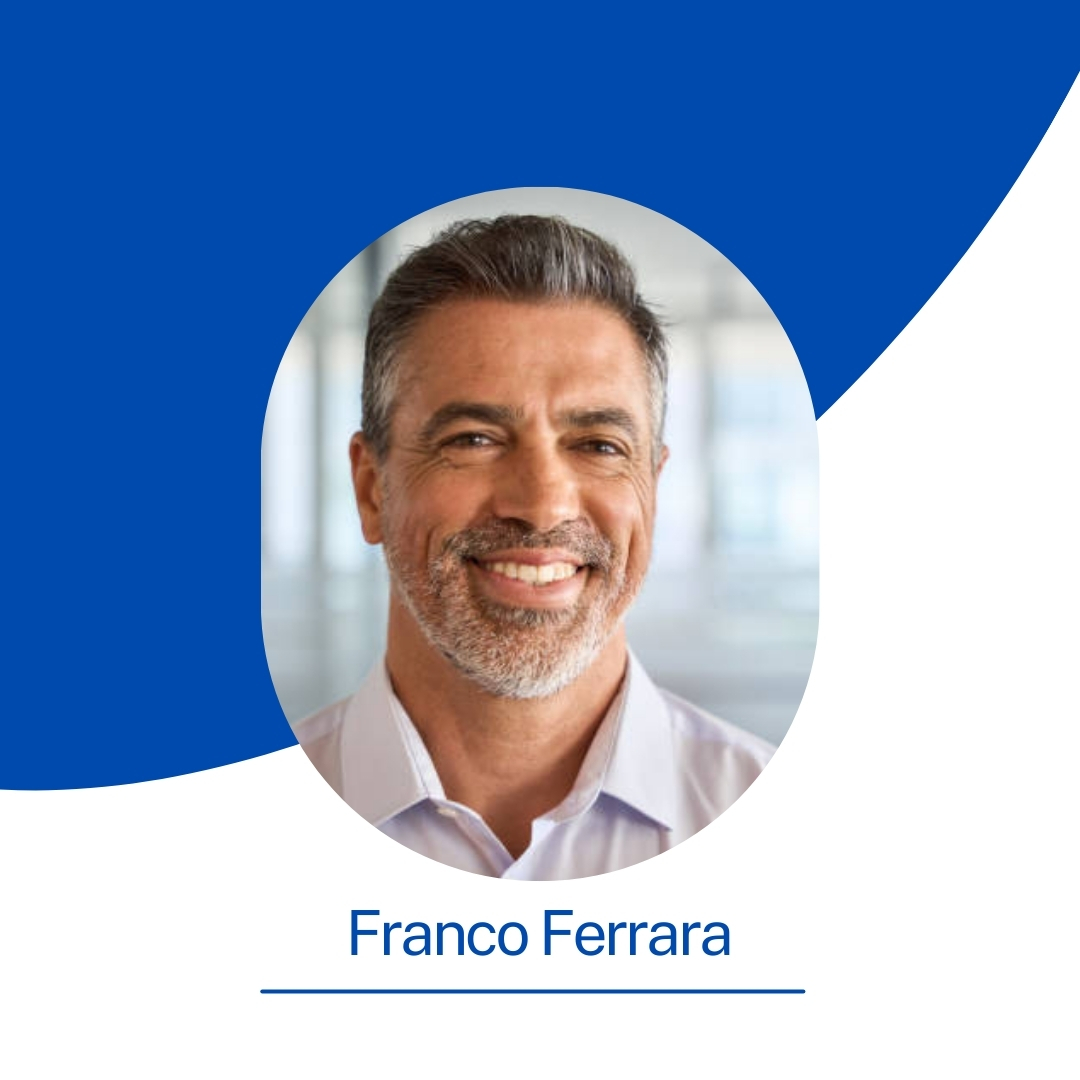
\includegraphics[height=10cm]{pics/FrancoPersona.jpg}
\end{figure}
\textbf{Profilo:}\\
Franco ha 50 anni, è titolare di un'agenzia immobiliare di medie dimensioni a Napoli con 5--8 agenti. Gestisce sia la parte operativa che quella amministrativa. Ha iniziato l'attività oltre 20 anni fa e cerca soluzioni digitali per modernizzare i processi senza stravolgere il lavoro quotidiano. Vuole strumenti semplici, affidabili e che riducano il carico amministrativo. Si aspetta dalla piattaforma un processo di registrazione chiaro e una dashboard semplice per gestire gli agenti.

\textbf{Obiettivi:}
\begin{itemize}[nosep]
  \item Registrare l'agenzia sulla piattaforma e configurare l'account iniziale.
  \item Creare account per i propri agenti in modo semplice e veloce.
  \item Monitorare il portafoglio immobili pubblicati dall'agenzia.
  \item Verificare le performance degli agenti (numero di annunci, recensioni ricevute).
\end{itemize}

\textbf{Motivazioni:}\\
Centralizzare i processi digitali dell'agenzia, migliorare la qualità del servizio verso i clienti, aumentare la visibilità complessiva dell'agenzia sul mercato.

\textbf{Competenze digitali:}\\
Medie. Utilizza computer per lavoro quotidiano, ma non è esperto di tecnologie avanzate. Preferisce soluzioni semplici e affidabili.

\textbf{Scenari tipici:}
\begin{itemize}[nosep]
  \item Registra l'agenzia tramite form dedicato con dati completi.
  \item Accede alla dashboard agenzia e visualizza panoramica degli agenti.
  \item Crea nuovi account agenti inserendo dati anagrafici e di contatto.
\end{itemize}

\textbf{Pain points:}
\begin{itemize}[nosep]
  \item Processo di registrazione iniziale troppo complesso o poco chiaro.
  \item Mancanza di dashboard chiara per monitorare le attività dell'agenzia.
\end{itemize}
\pagebreak

\section{Attori e casi d’uso}

\subsection{Attori}

\begin{itemize}[nosep]
  \item \textbf{Visitatore}: utente non autenticato che può cercare e visualizzare immobili e profili agenti.
  \item \textbf{Cliente}: utente registrato interessato a servizi immobiliari.
  \item \textbf{Agente immobiliare}: utente con ruolo professionale associato a un’agenzia.
  \item \textbf{Manager di agenzia}: utente che registra e gestisce un’agenzia e i relativi agenti.
  \item \textbf{Provider OAuth2 esterno}: Google, Facebook, GitHub.
\end{itemize}

\subsection{Elenco principali casi d’uso}

\begin{itemize}[nosep]
  \item UC01 -- Registrazione utente.
  \item UC02 -- Login utente.
  \item UC03 -- Login con account esterno (Google/Facebook/GitHub).
  \item UC04 -- Registrazione di una nuova agenzia.
  \item UC05 -- Creazione account agente da parte del manager.
  \item UC06 -- Ricerca avanzata di immobili (filtri + mappa).
  \item UC07 -- Visualizzazione dettaglio immobile.
  \item UC08 -- Creazione di un nuovo immobile (agente).
  \item UC09 -- Gestione profilo utente.
  \item UC10 -- Gestione profilo agente (biografia, foto profilo).
  \item UC11 -- Visualizzazione profilo agente con immobili e recensioni.
  \item UC12 -- Inserimento recensione su un agente.
  \item UC13 -- Visualizzazione elenco agenti.
\end{itemize}
\pagebreak
\subsubsection*{Use Case Diagrams}

I casi d'uso sopra elencati sono modellati tramite Use Case Diagram UML:
\\
\\
\begin{figure}[H]
    \centering
    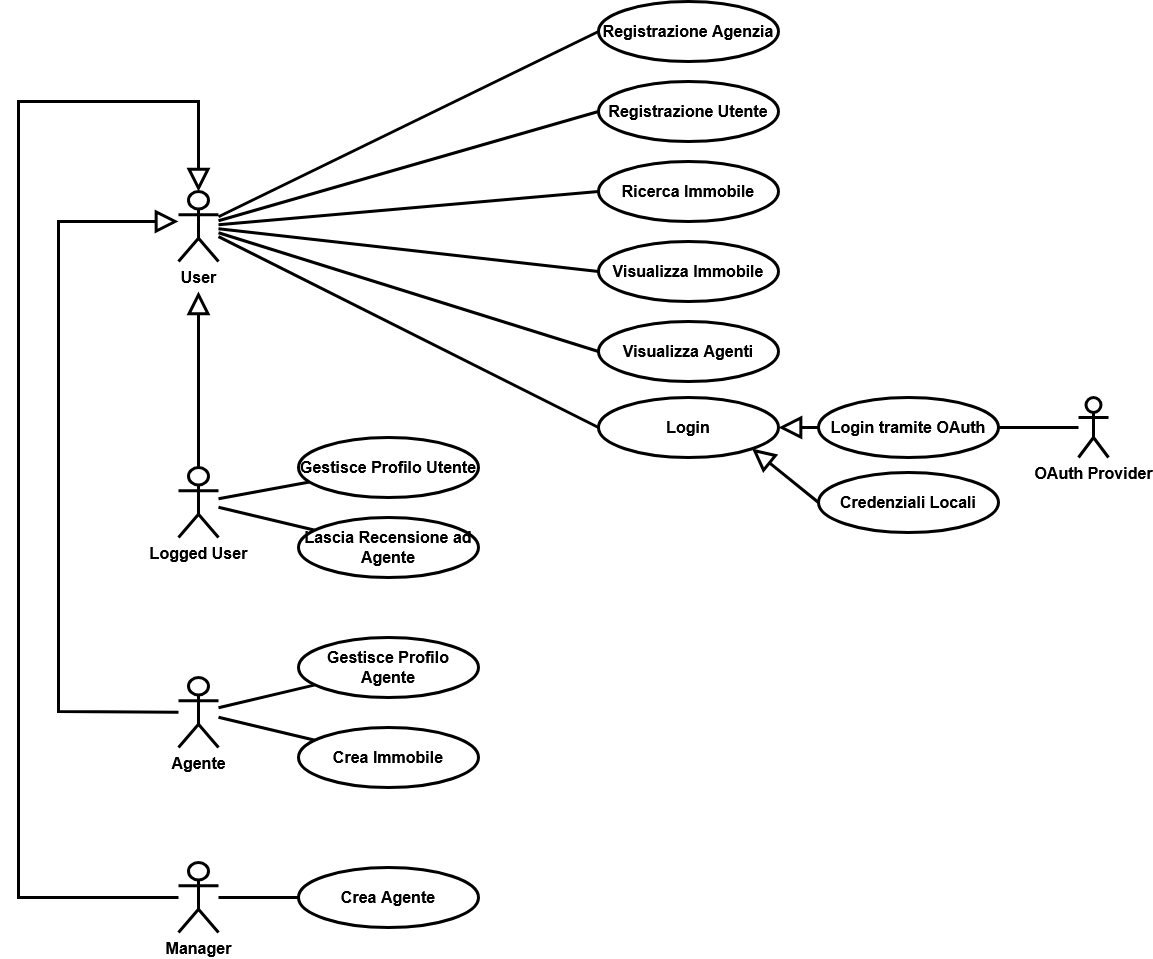
\includegraphics[width=\textwidth]{pics/UseCase.png}
    \caption{Use Case Diagram}
\end{figure}
\pagebreak

\section{Requisiti funzionali}

\begin{itemize}[nosep]
  \item \textbf{RF-01 -- Registrazione utente cliente}\\
  Un utente può registrarsi con e-mail e password (endpoint \texttt{/auth/register}).

  \item \textbf{RF-02 -- Registrazione agenzia + manager}\\
  Un manager registra l’agenzia e il proprio account manager (endpoint \texttt{/auth/register/agency}).

  \item \textbf{RF-03 -- Login con credenziali locali}\\
  Login con e-mail/password, ricezione JWT, accesso ad API protette (endpoint \texttt{/auth/login}).

  \item \textbf{RF-04 -- Login tramite provider esterno}\\
  Accesso tramite Google, Facebook, GitHub (flusso OAuth2 configurato in \texttt{application.properties}).

  \item \textbf{RF-05 -- Creazione account agente}\\
  Il manager di agenzia crea account agenti associati alla propria agenzia.

  \item \textbf{RF-06 -- Creazione annuncio immobile}\\
  Un agente autenticato crea un immobile completo di dettagli, servizi, foto e posizione.

  \item \textbf{RF-07 -- Ricerca avanzata immobili}\\
  L’utente può cercare immobili usando filtri multipli: città, tipo, prezzo, stanze, metri quadri, piano, bagni, classe energetica, agente.

  \item \textbf{RF-08 -- Ricerca geografica a raggio}\\
  L’utente può selezionare un punto sulla mappa e un raggio per limitare la ricerca.

  \item \textbf{RF-09 -- Visualizzazione immobili su mappa}\\
  I risultati vengono mostrati anche su una mappa interattiva (Google Maps).

  \item \textbf{RF-10 -- Gestione profilo utente}\\
  L’utente autenticato modifica dati personali e password.

  \item \textbf{RF-11 -- Gestione profilo agente}\\
  L’agente aggiorna biografia e foto profilo, oltre ai propri dati personali.

  \item \textbf{RF-12 -- Visualizzazione profilo agente}\\
  L’utente consulta dati agenti, immobili associati e recensioni.

  \item \textbf{RF-13 -- Inserimento recensione agente}\\
  Un cliente autenticato inserisce una recensione (punteggio + commento) per un agente.

\end{itemize}

\section{Requisiti non funzionali}

\begin{itemize}[nosep]
  \item \textbf{RNF-01 -- Prestazioni}\\
  Le ricerche immobili devono completarsi in meno di un secondo dataset realistici.

  \item \textbf{RNF-02 -- Scalabilità}\\
  Architettura back-end stateless, sessioni gestite tramite JWT, possibilità di scalare orizzontalmente.

  \item \textbf{RNF-03 -- Sicurezza}\\
  Password memorizzate come hash sicuri; JWT firmati con chiave segreta; integrazione OAuth2; ruoli e autorizzazioni.

  \item \textbf{RNF-04 -- Affidabilità}\\
  Gestione centralizzata delle eccezioni; presenza di test unitari e di integrazione.

  \item \textbf{RNF-05 -- Usabilità}\\
  UI responsiva, flussi chiari per ricerca, login, gestione profilo; messaggi di errore espliciti.

  \item \textbf{RNF-06 -- Manutenibilità}\\
  Separazione in livelli (Controller, Service, Repository, DTO, Model); uso di convenzioni standard.

  \item \textbf{RNF-07 -- Portabilità}\\
  Utilizzo di Docker; dipendenze configurabili tramite variabili d’ambiente.
\end{itemize}

\section{Requisiti di dominio}

\begin{itemize}[nosep]
  \item Supporto a tipologie di inserzione \texttt{SALE} e \texttt{RENT}, con previsione di estensione a affitti brevi/case vacanze.
  \item Ogni immobile è associato a un agente, un’agenzia, servizi (amenities), foto e ad una posizione geografica (punto).
  \item Gli utenti possono avere più ruoli; agenti e manager sono associati a un’agenzia.
  \item Le recensioni sono legate a un singolo agente e, opzionalmente, a un utente cliente.
\end{itemize}


\section{MockUp dei casi d'uso}
Di seguito sono riportati i mock up per i casi di uso e le loro estensioni.
\subsection{M0: Login Page}

\begin{figure}[H]
    \centering
    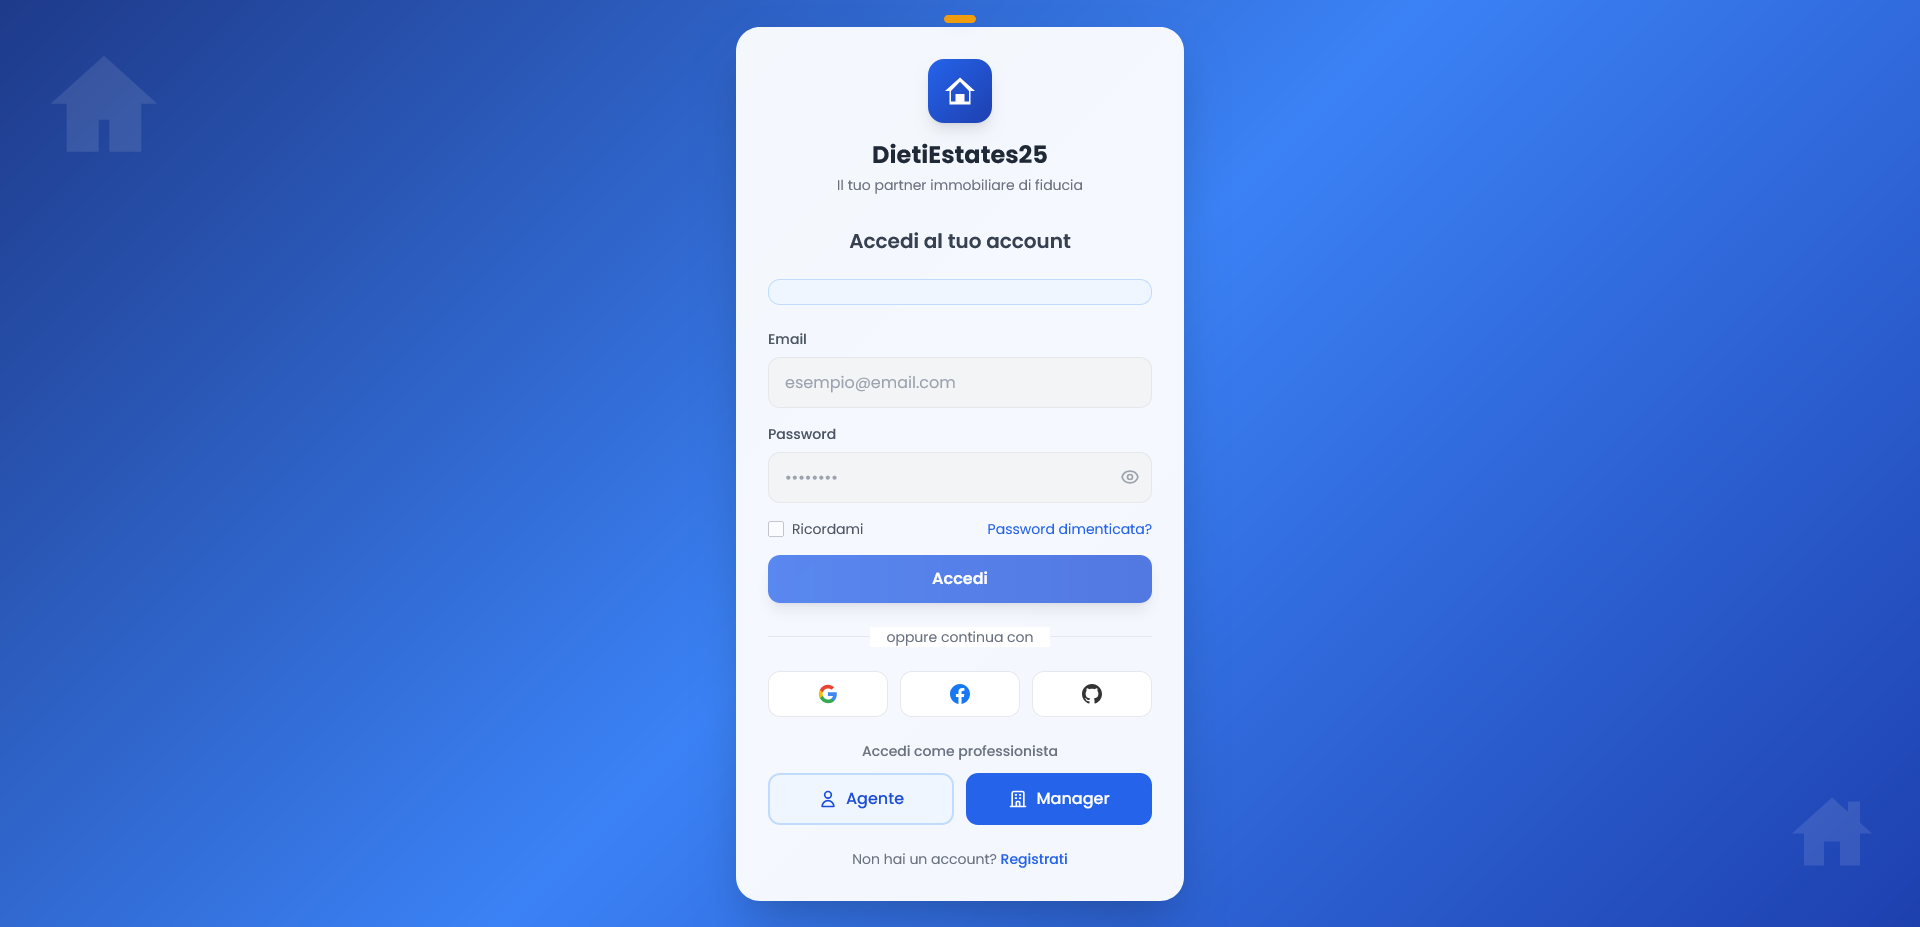
\includegraphics[width=\textwidth]{pics/LoginMU.png}
    \caption{Login Page}
\end{figure}

\subsection{M1: Landing Page}
\begin{figure}[H]
    \centering
    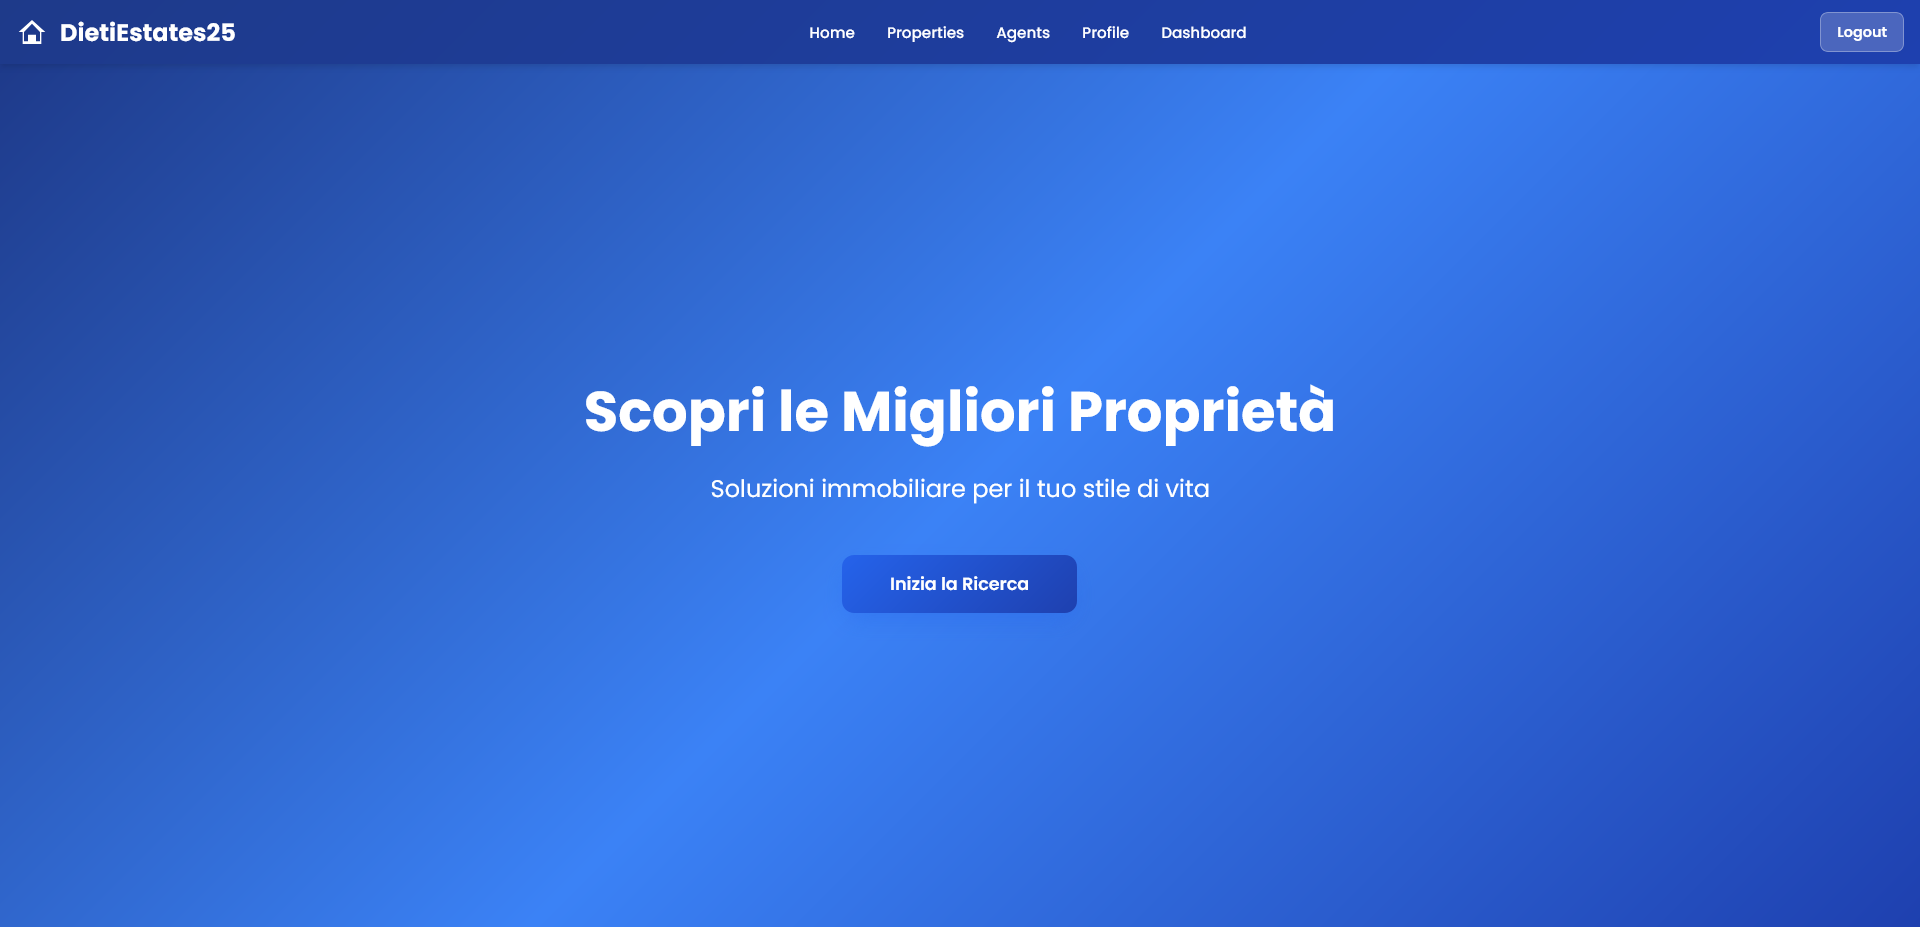
\includegraphics[width=\textwidth]{pics/LandingPage.png}
    \caption{Landing Page}
\end{figure}

\subsection{M2: Pagina di Ricerca}

\begin{figure}[H]
    \centering
    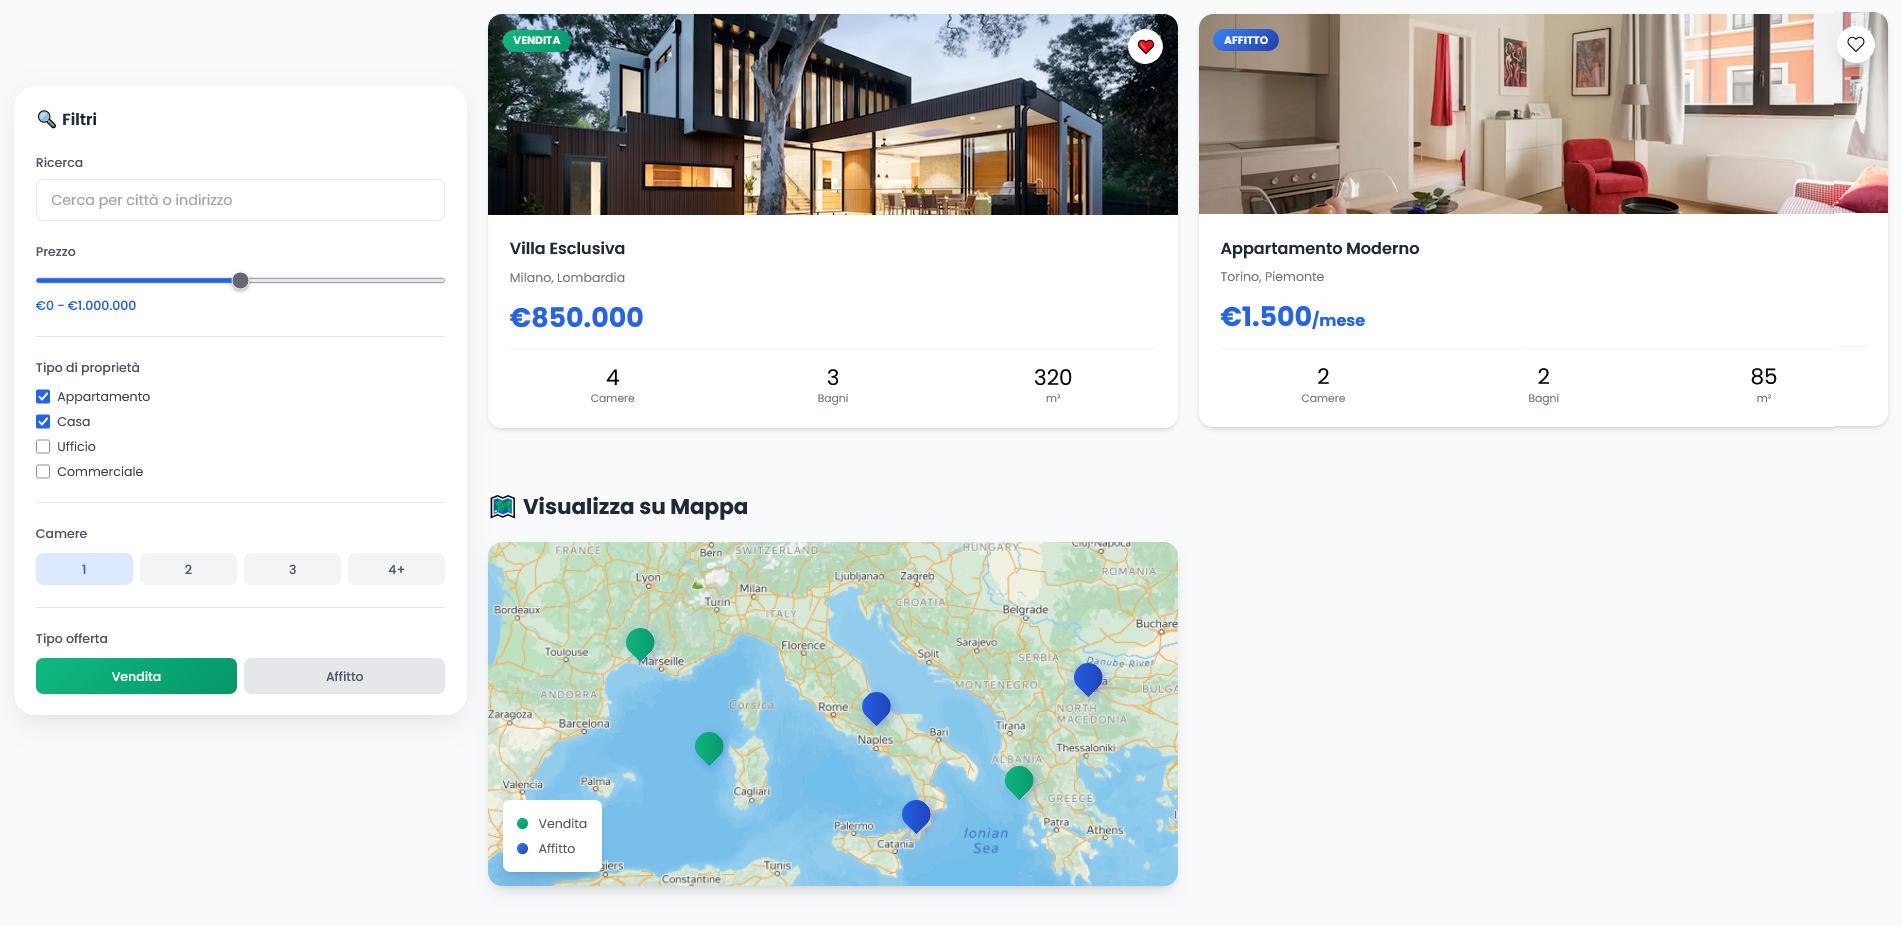
\includegraphics[width=\textwidth]{pics/RicercaMU.png}
    \caption{Pagina di Ricera}
\end{figure}


\subsection{M3: Ricerca Senza Risultati}

\begin{figure}[H]
    \centering
    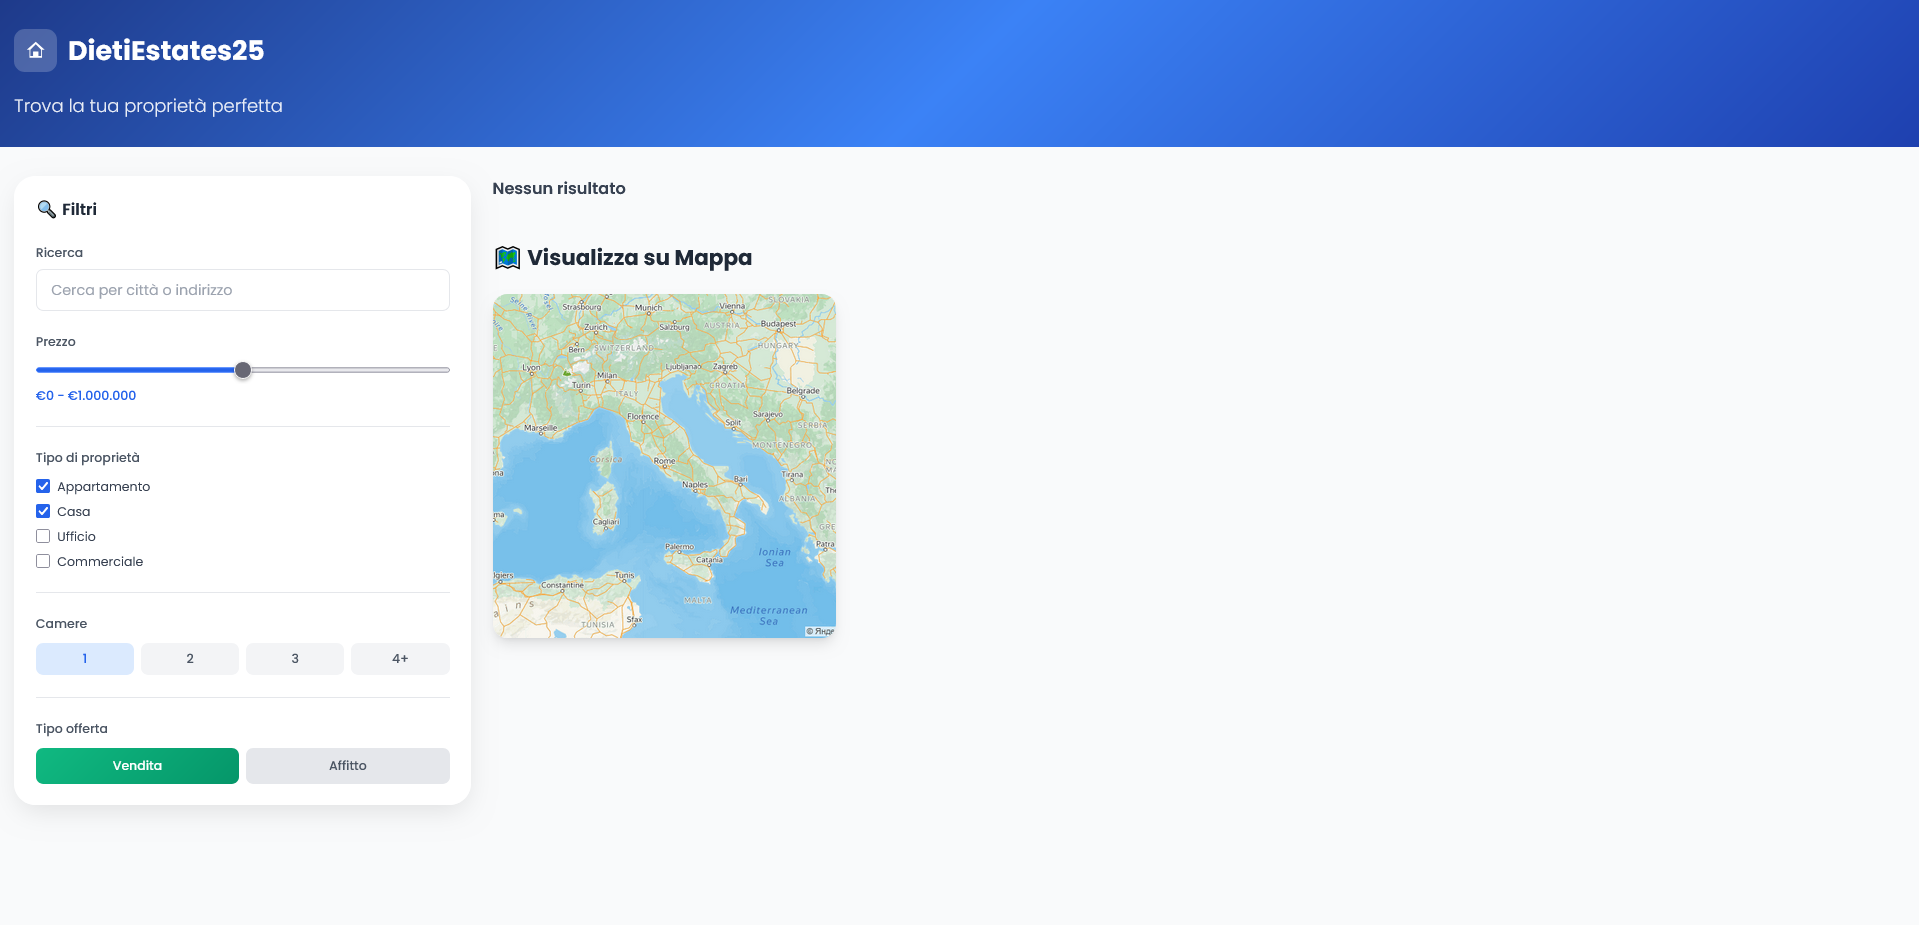
\includegraphics[width=\textwidth]{pics/RicercaNoResultsMU.png}
    \caption{Ricerca Senza Risultati}
\end{figure}

\subsection{M4: Dashboard}

\begin{figure}[H]
    \centering
    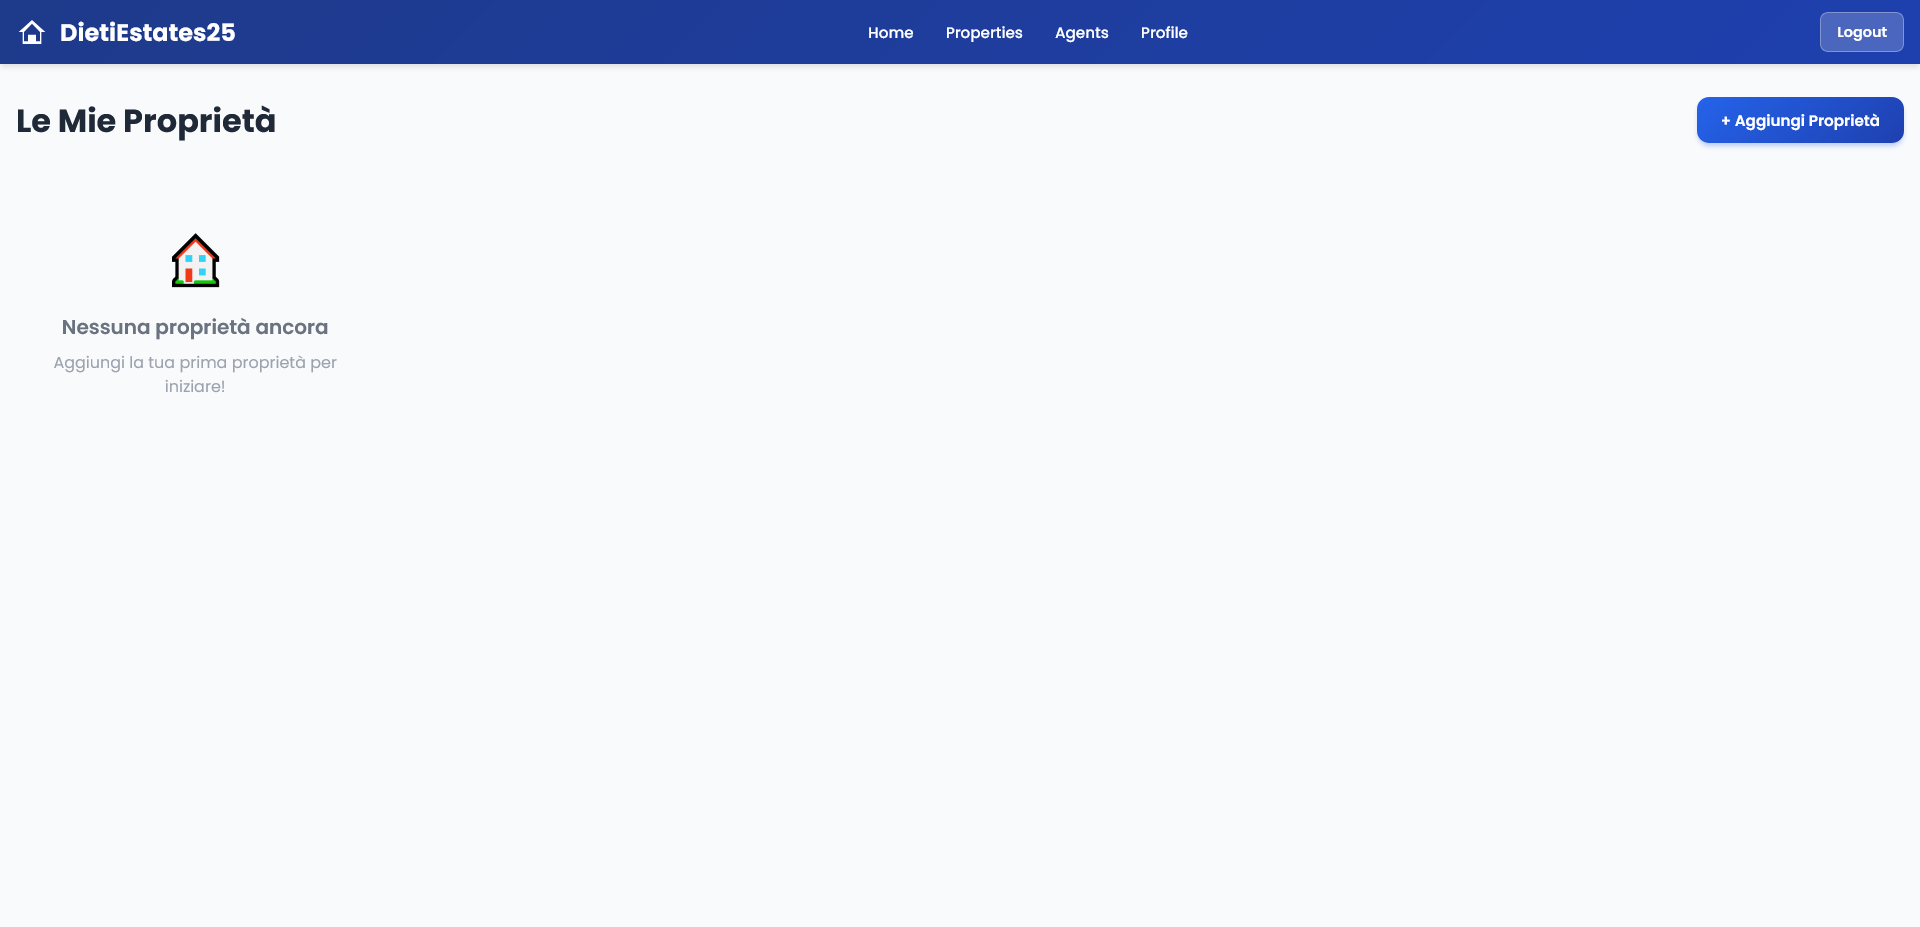
\includegraphics[width=\textwidth]{pics/dashboardMU.png}
    \caption{Dashboard}
\end{figure}

\subsection{M5: Creazione Immobile}

\begin{figure}[H]
    \centering
    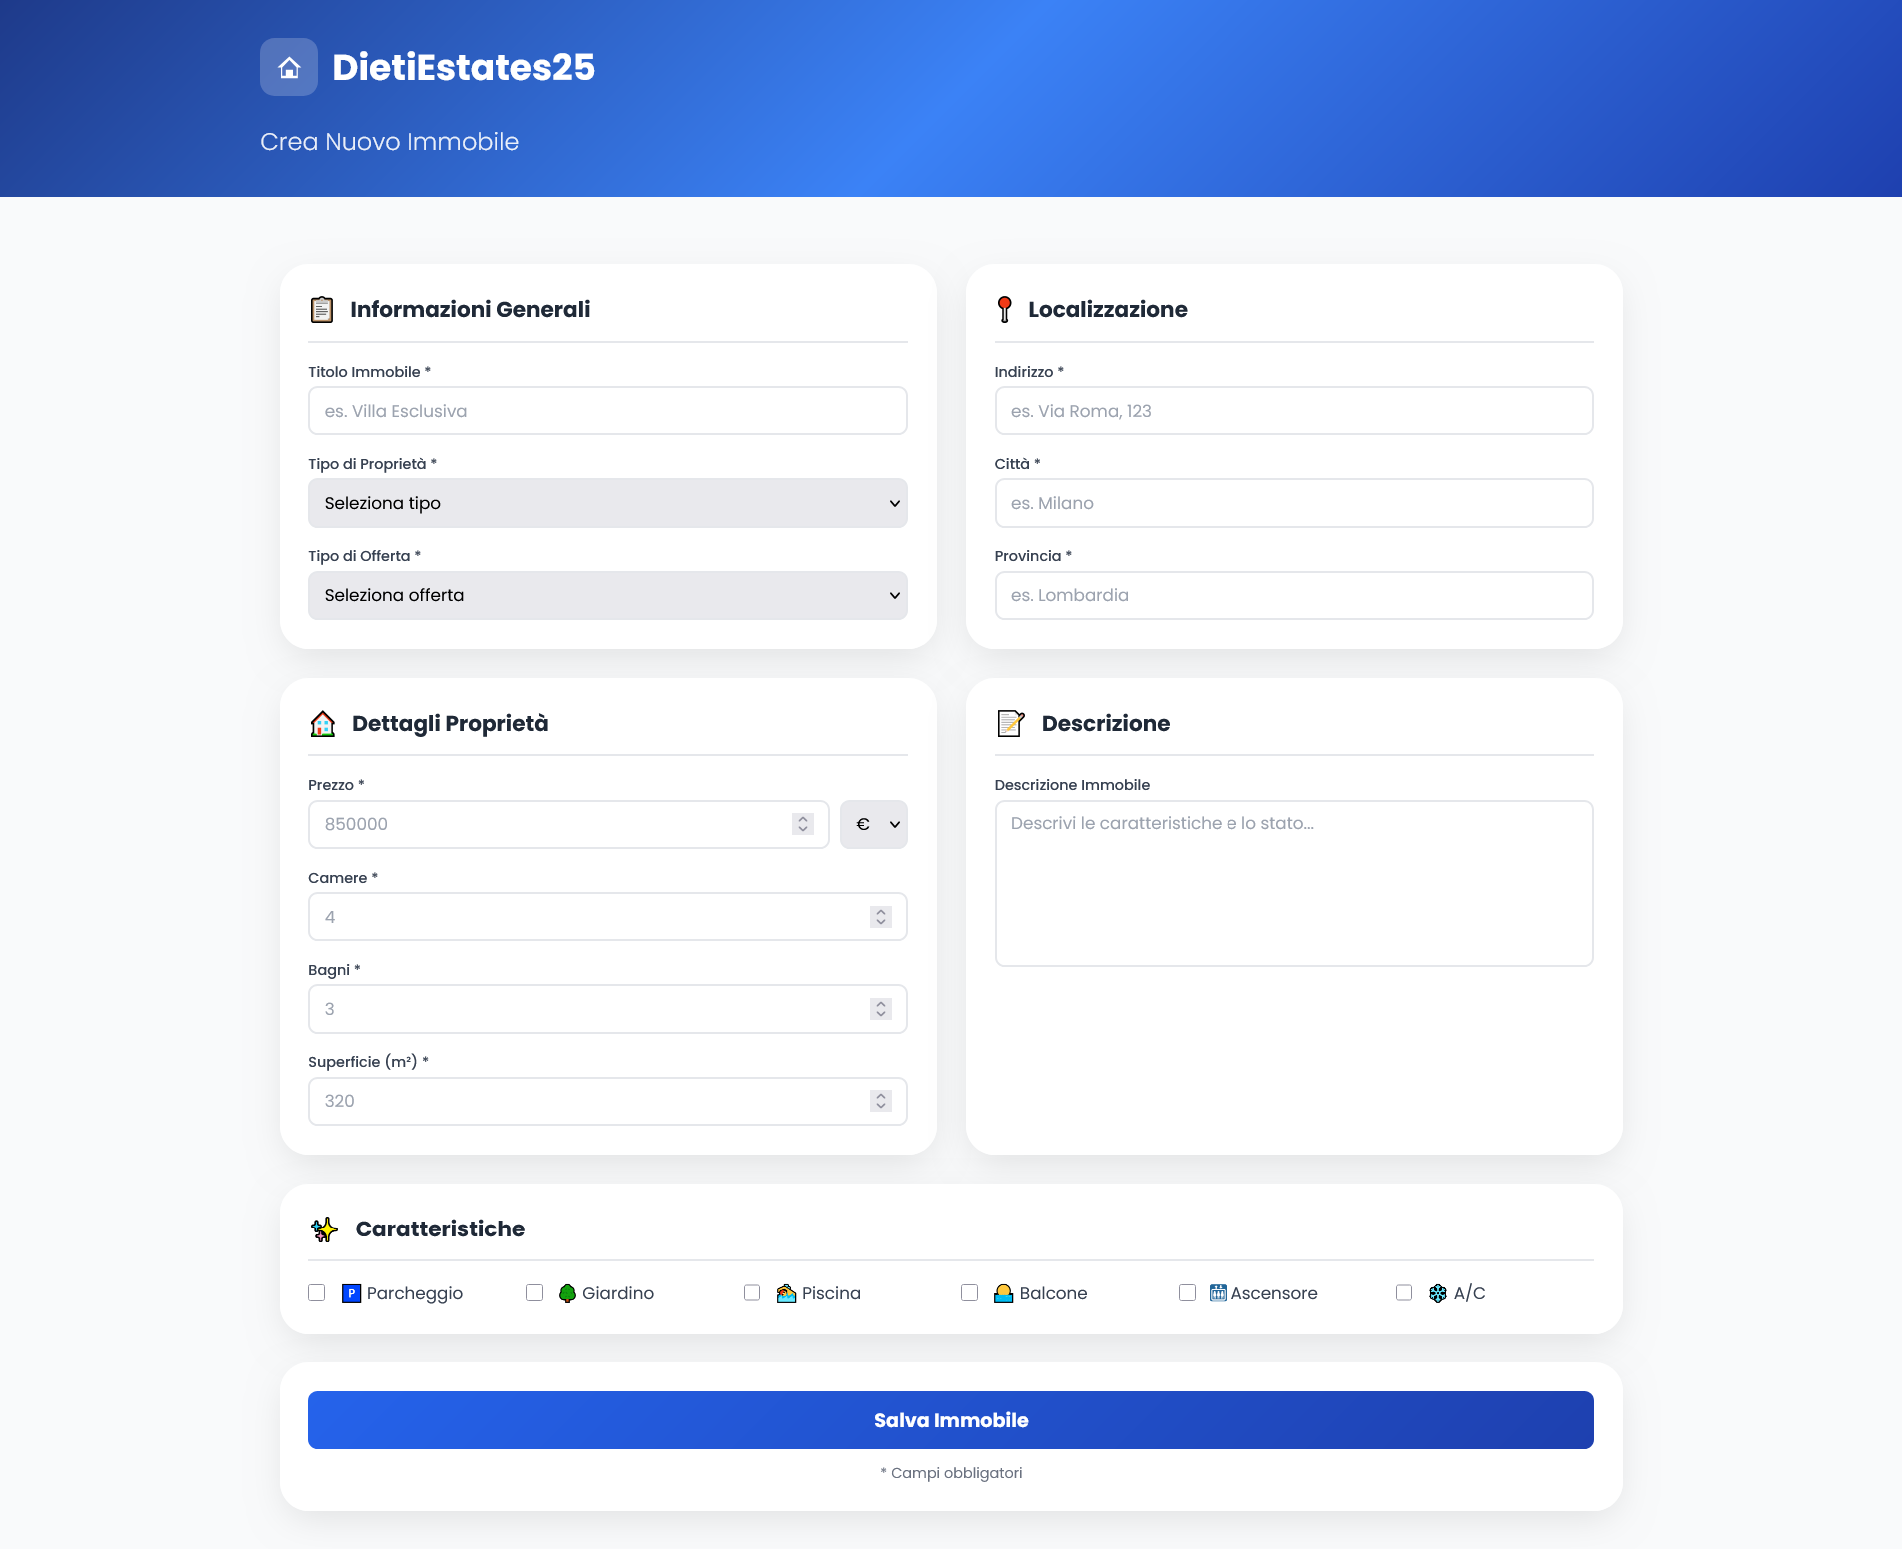
\includegraphics[width=\textwidth]{pics/CreaMU.png}
    \caption{Creazione Immobile}
\end{figure}


\subsection{M6: Creazione Immobile - Campi Incompleti}

\begin{figure}[H]
    \centering
    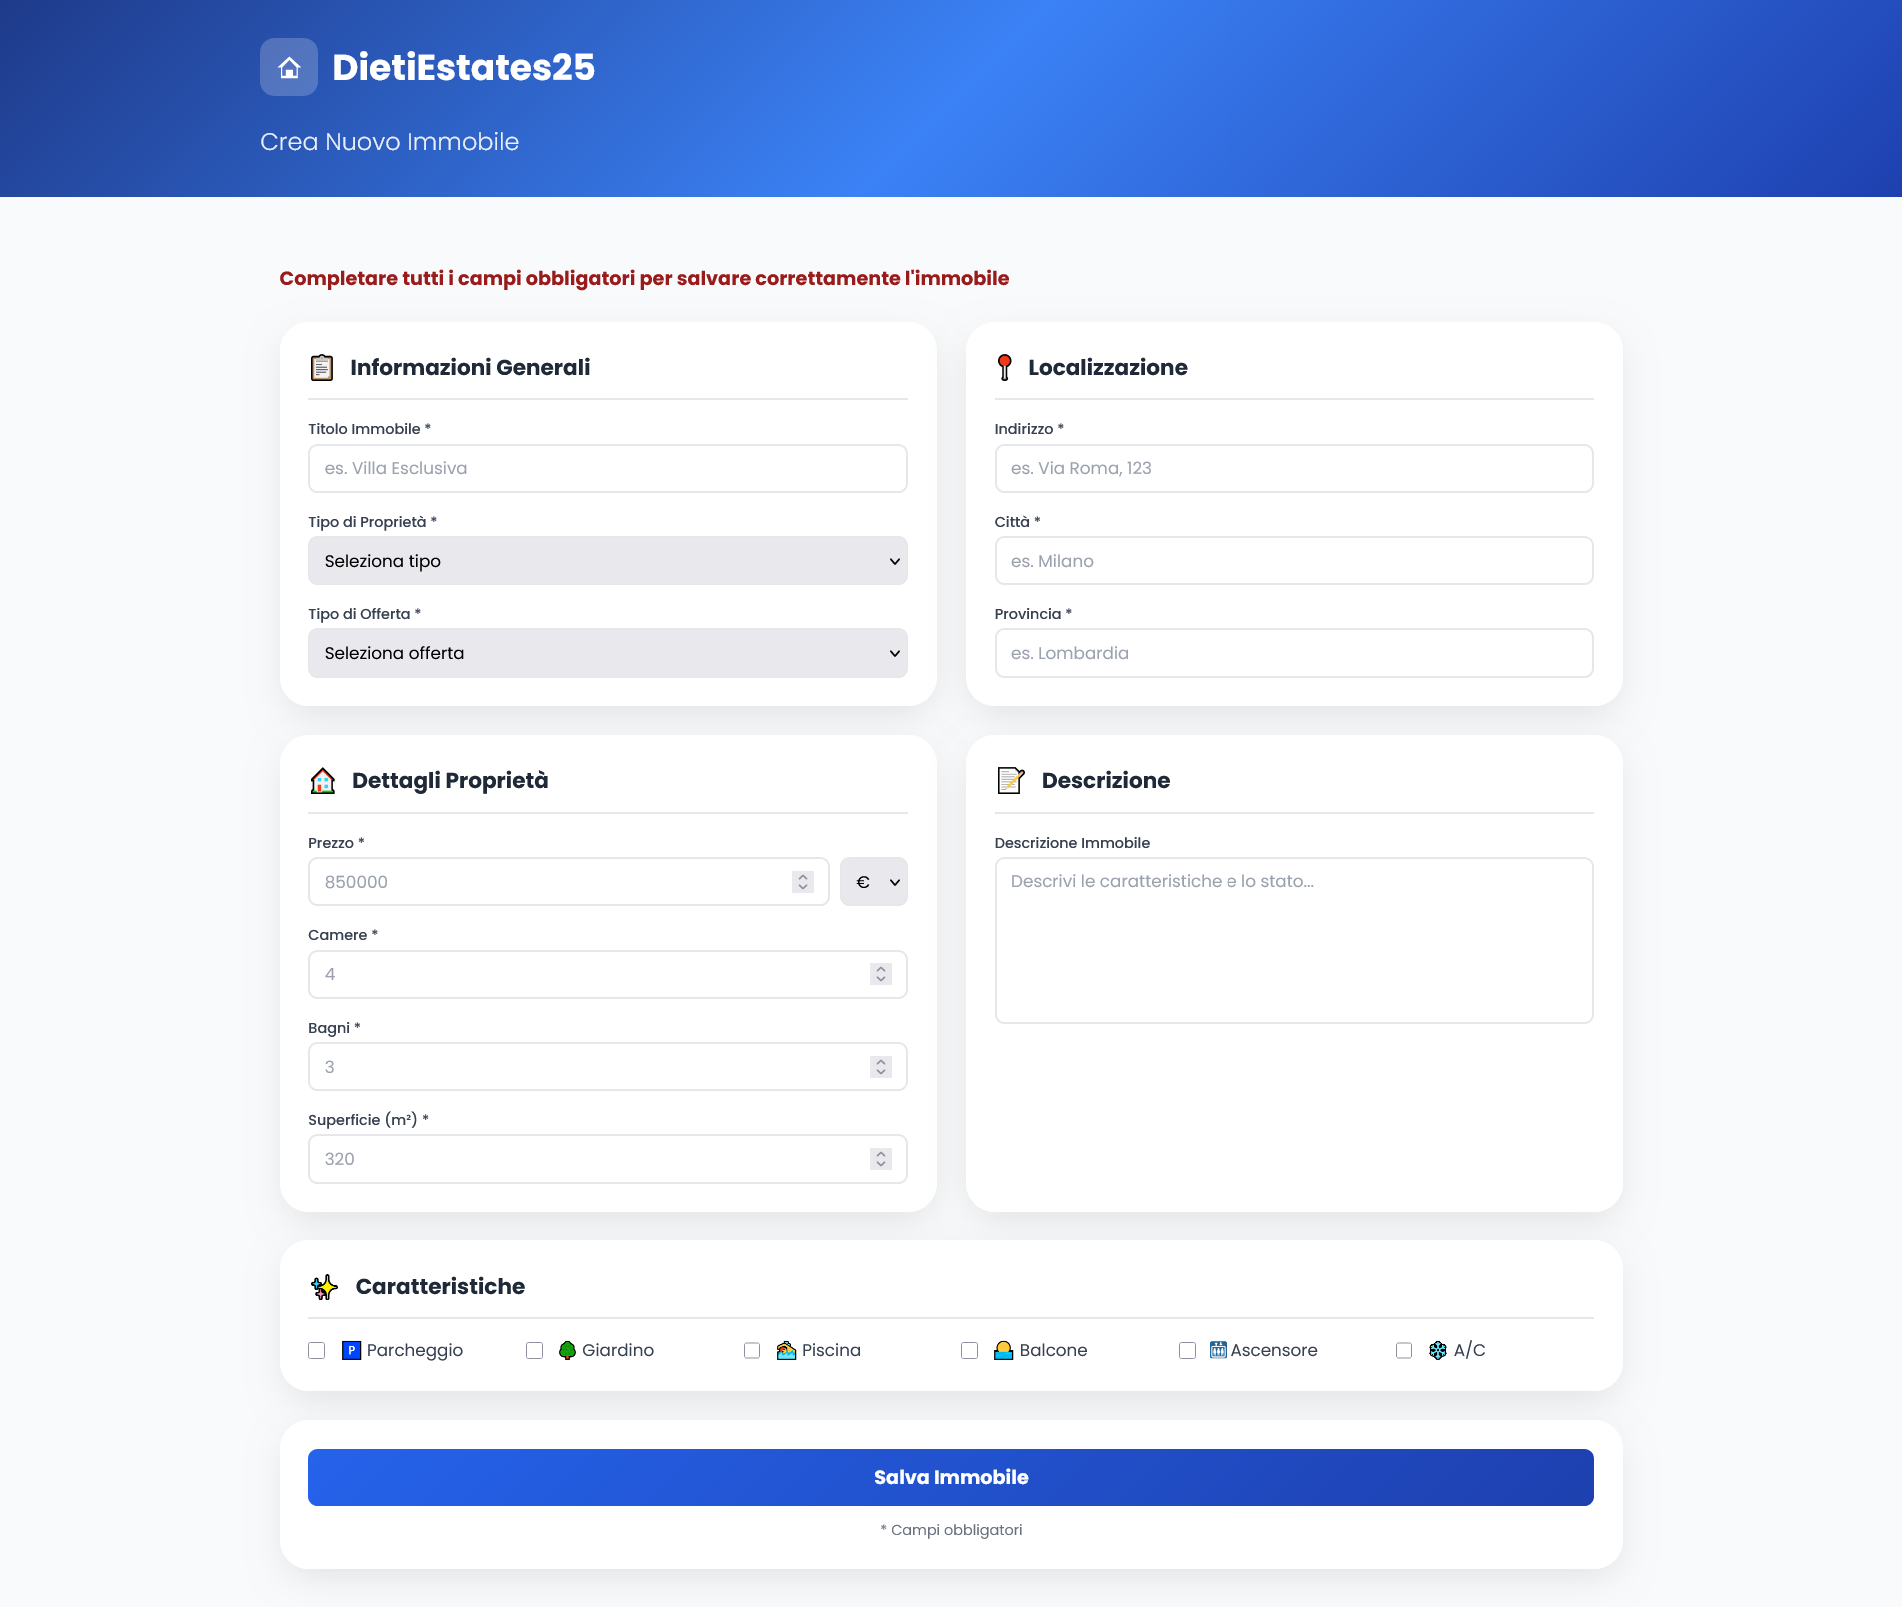
\includegraphics[width=\textwidth]{pics/CreaErrMU.png}
    \caption{M5: Creazione Immobile - Campi Incompleti}
\end{figure}

\subsection{M7: Pagina di Profilo}

\begin{figure}[H]
    \centering
    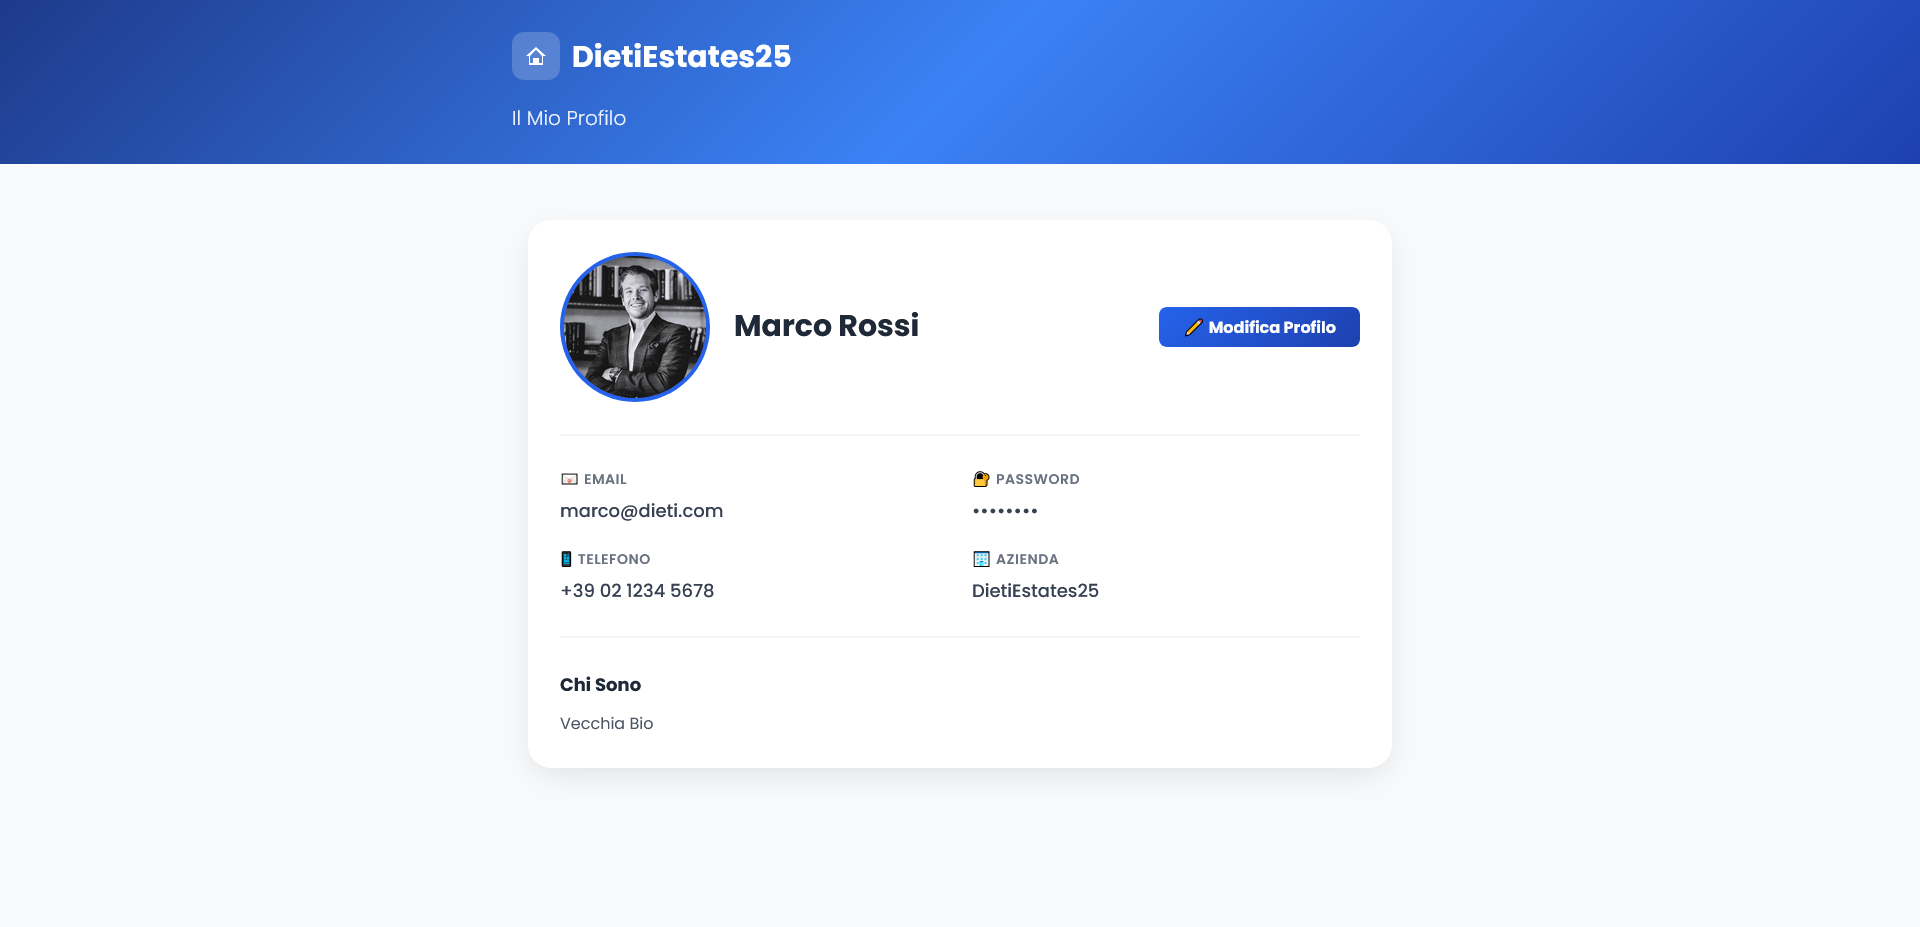
\includegraphics[width=\textwidth]{pics/ProfilePage.png}
    \caption{Pagina di Profilo}
\end{figure}

\subsection{M8: Modifica in Corso}

\begin{figure}[H]
    \centering
    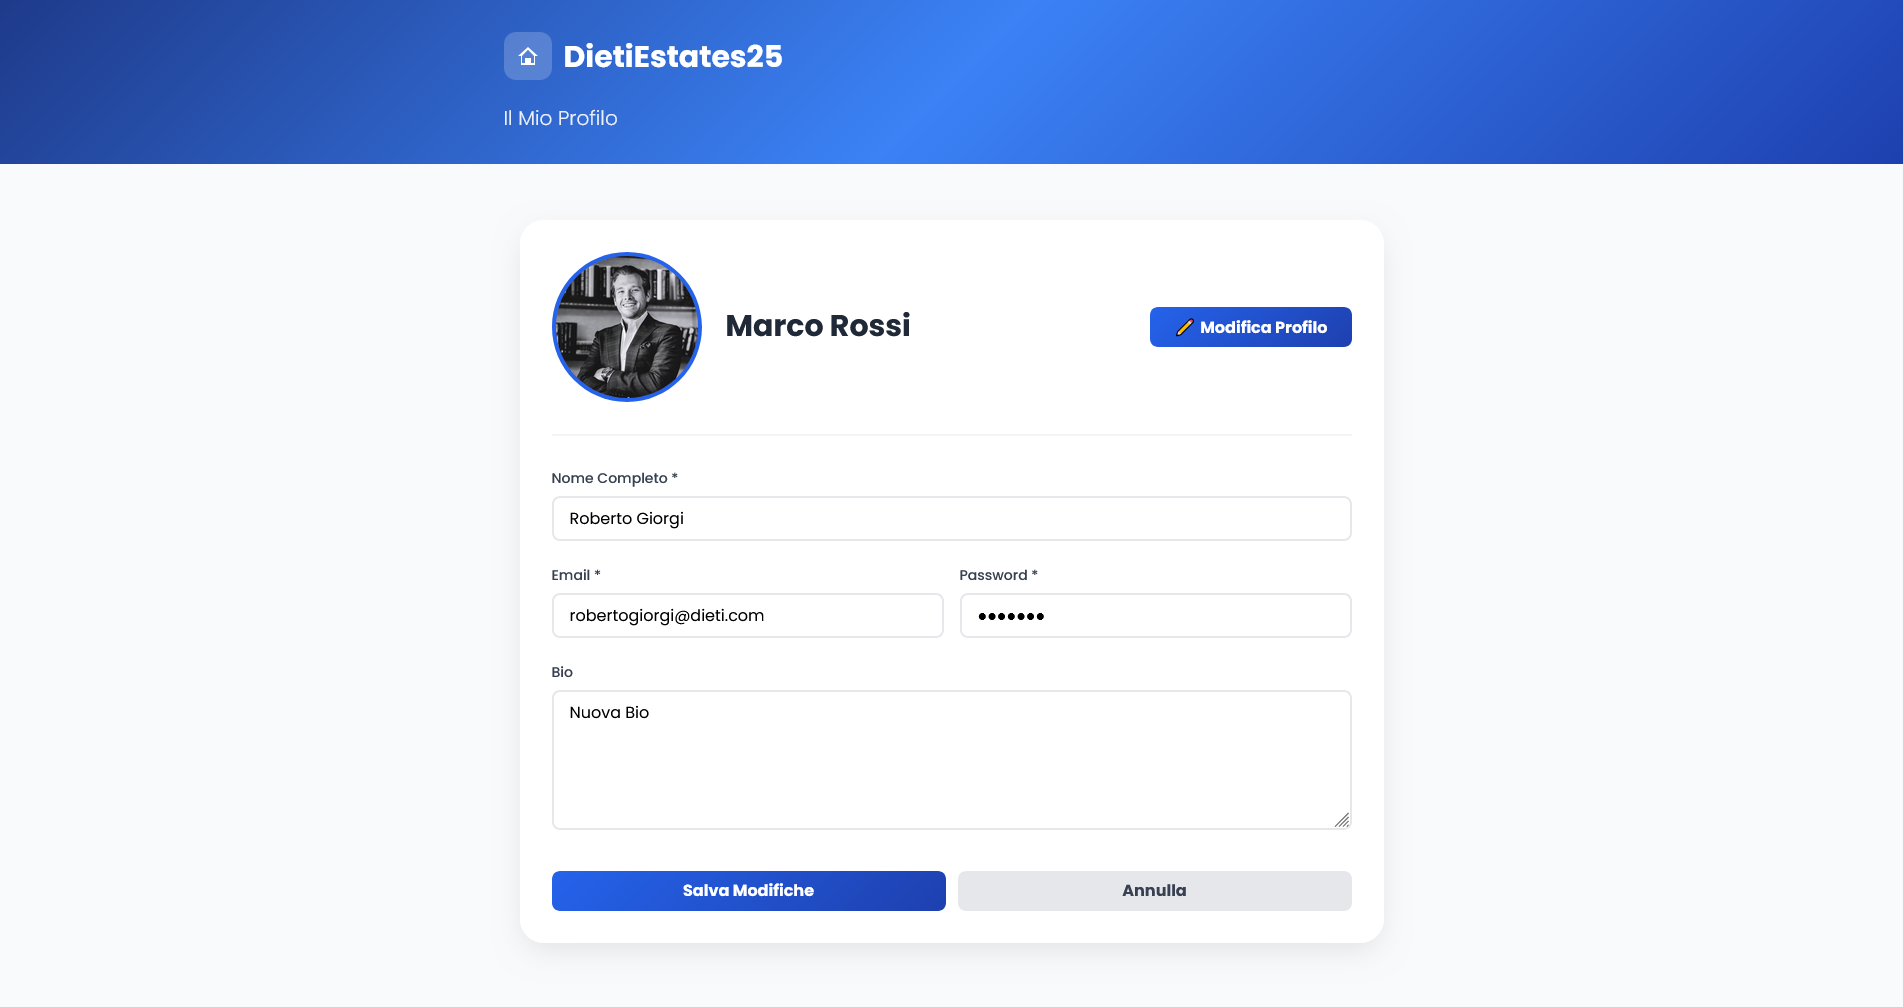
\includegraphics[width=\textwidth]{pics/ProfileModify.png}
    \caption{Modifica in Corso}
\end{figure}

\subsection{M9: Modifica con Successo}

\begin{figure}[H]
    \centering
    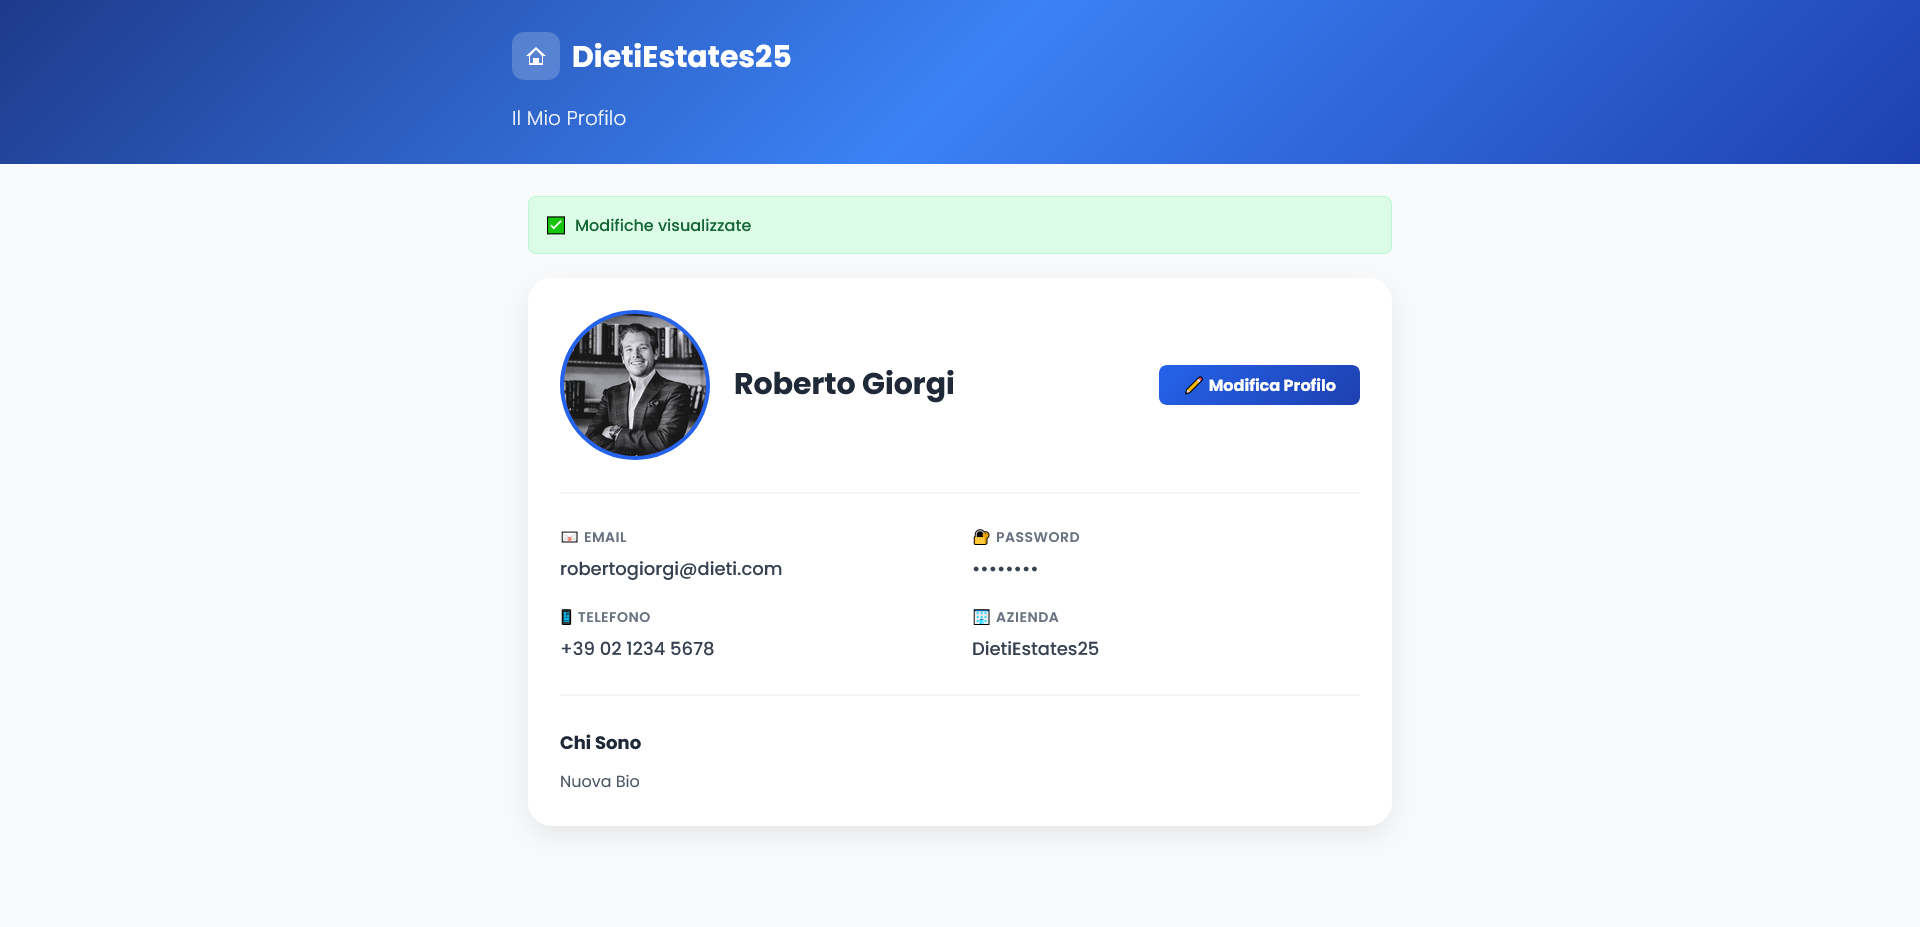
\includegraphics[width=\textwidth]{pics/ModifySuccess.png}
    \caption{Modifica con Successo}
\end{figure}

\subsection{M10: Pagina di Dettaglio Agente}

\begin{figure}[H]
    \centering
    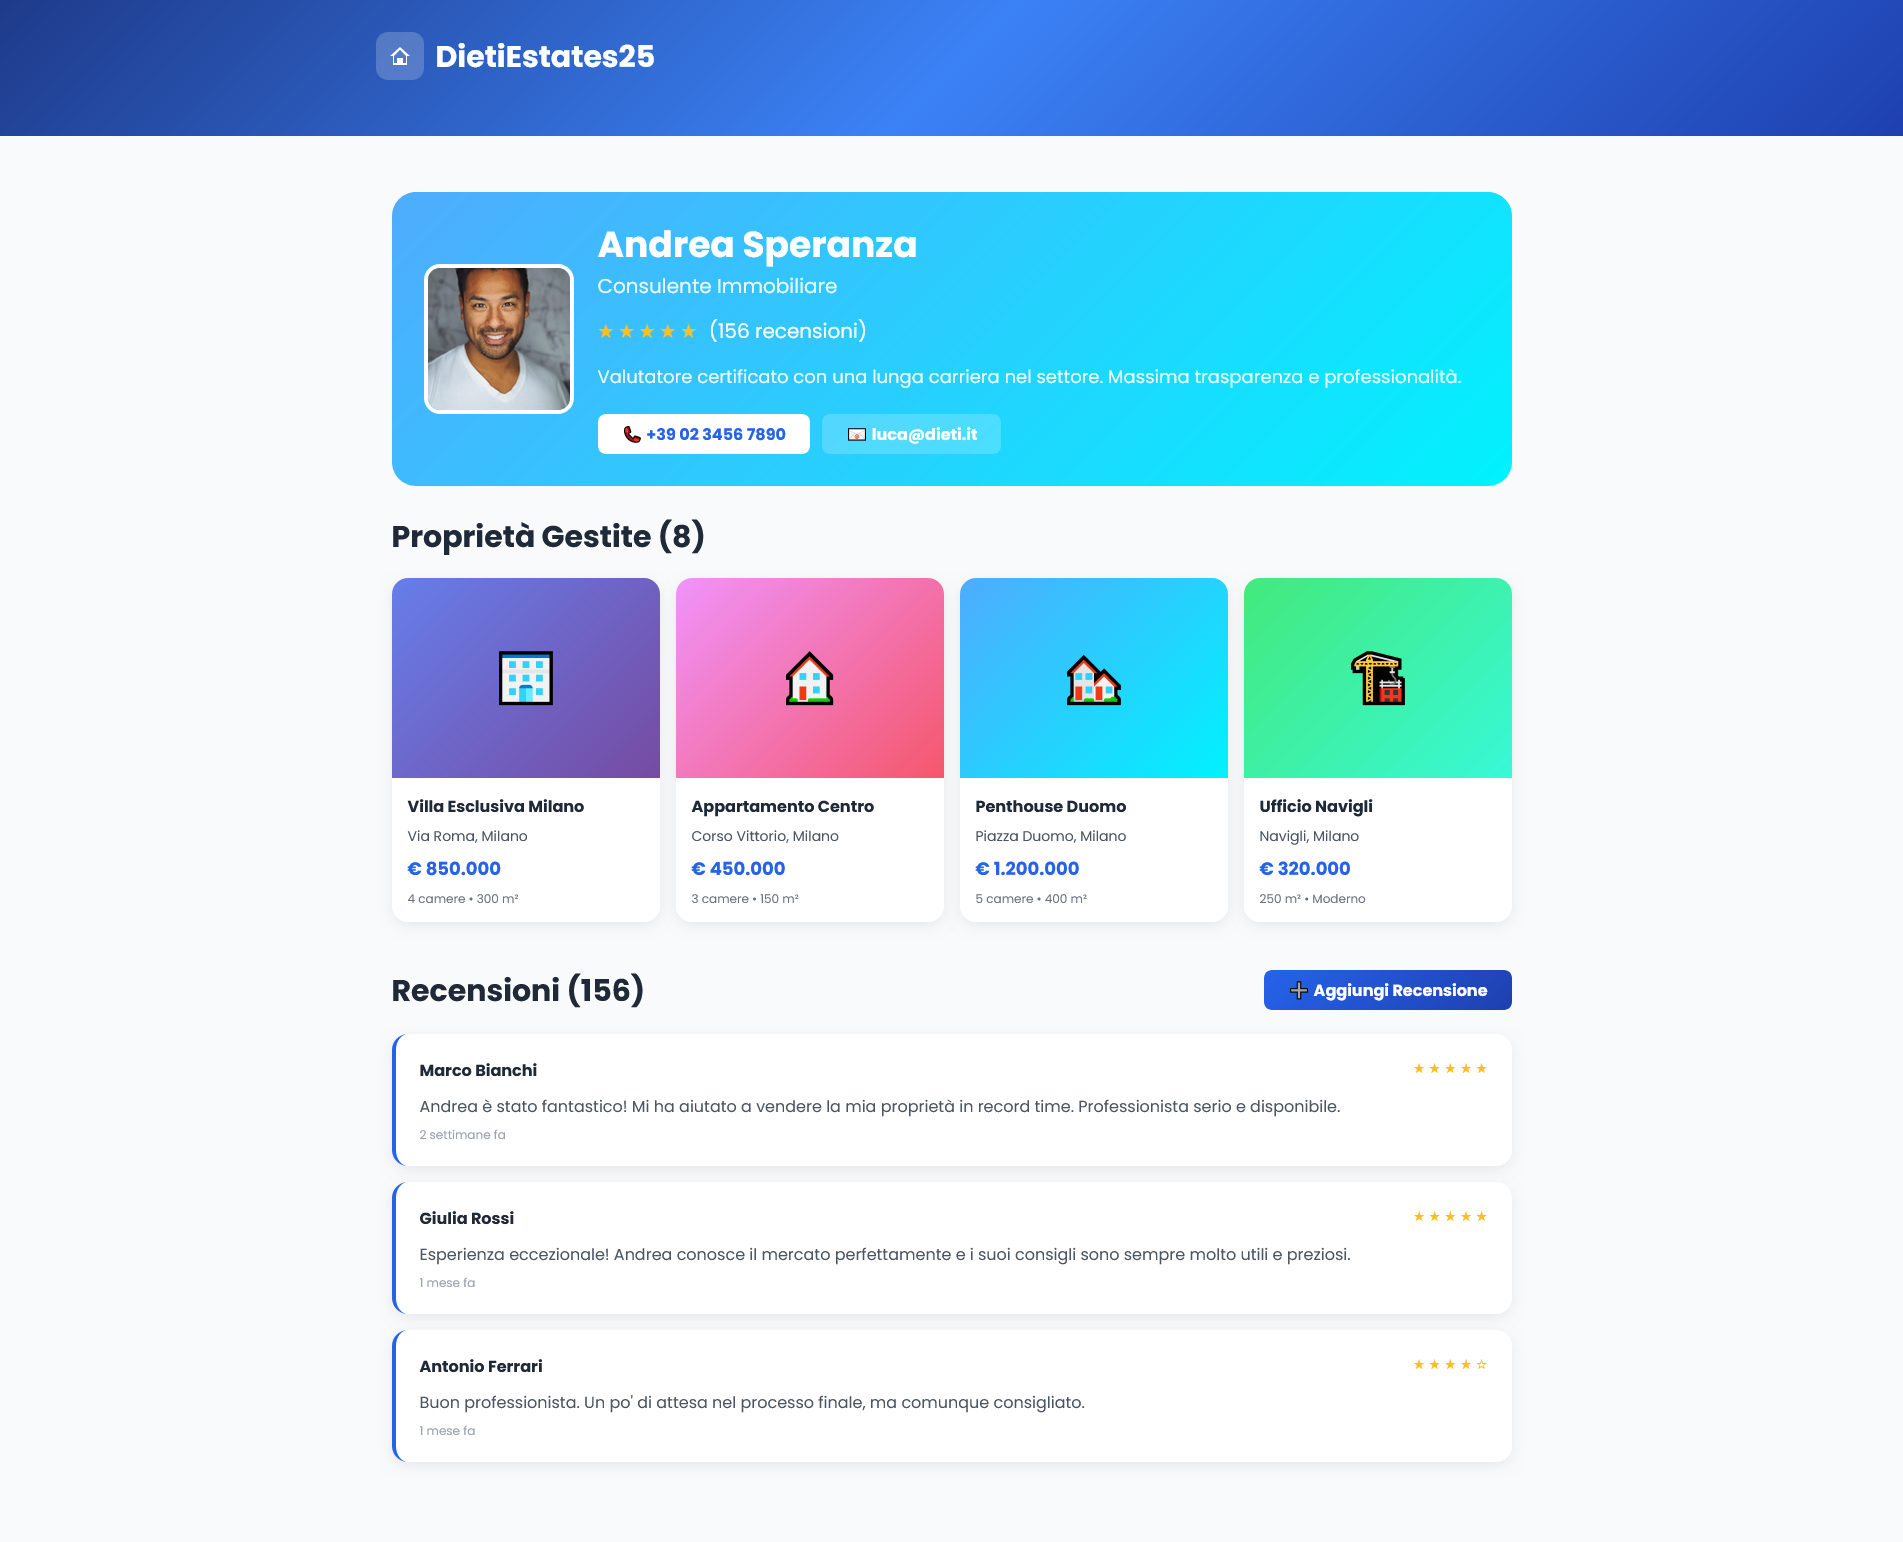
\includegraphics[width=\textwidth]{pics/AgentDetail.png}
    \caption{Pagina di Dettaglio Agente}
\end{figure}

\subsection{M11: Aggiunta Recensione}

\begin{figure}[H]
    \centering
    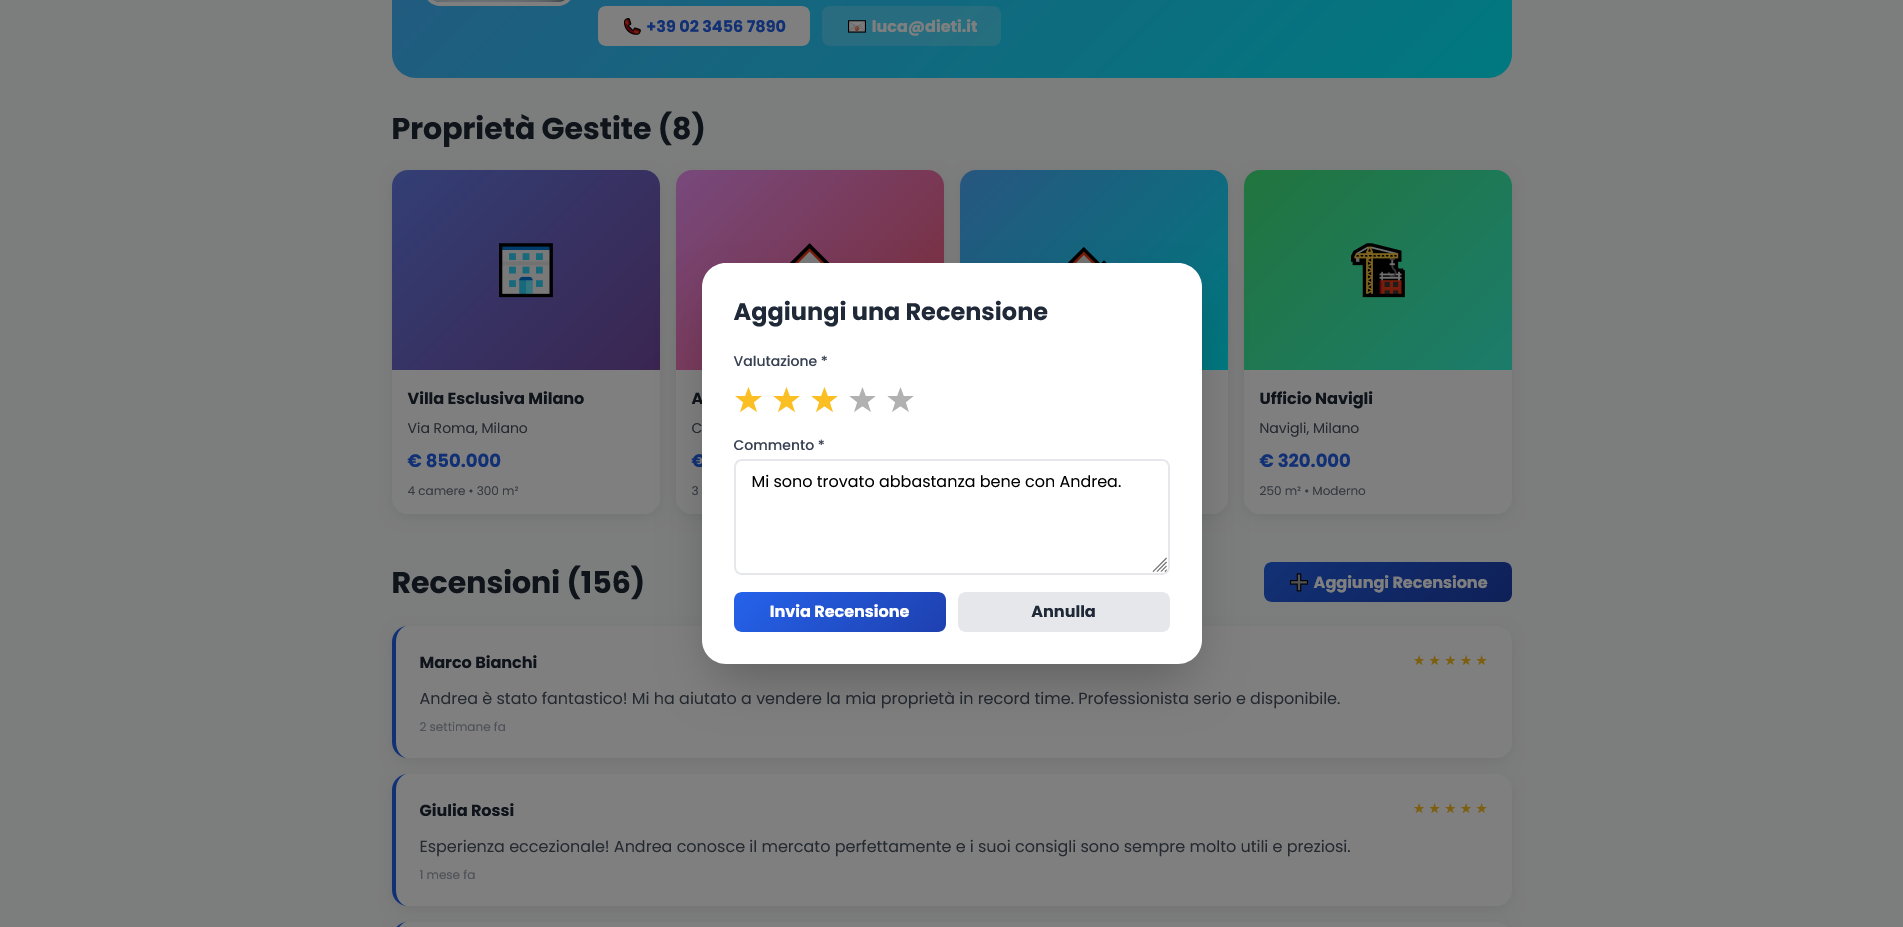
\includegraphics[width=\textwidth]{pics/ReviewDetail.png}
    \caption{Aggiunta Recensione}
\end{figure}

\subsection{M12: Recensione Aggiunta}

\begin{figure}[H]
    \centering
    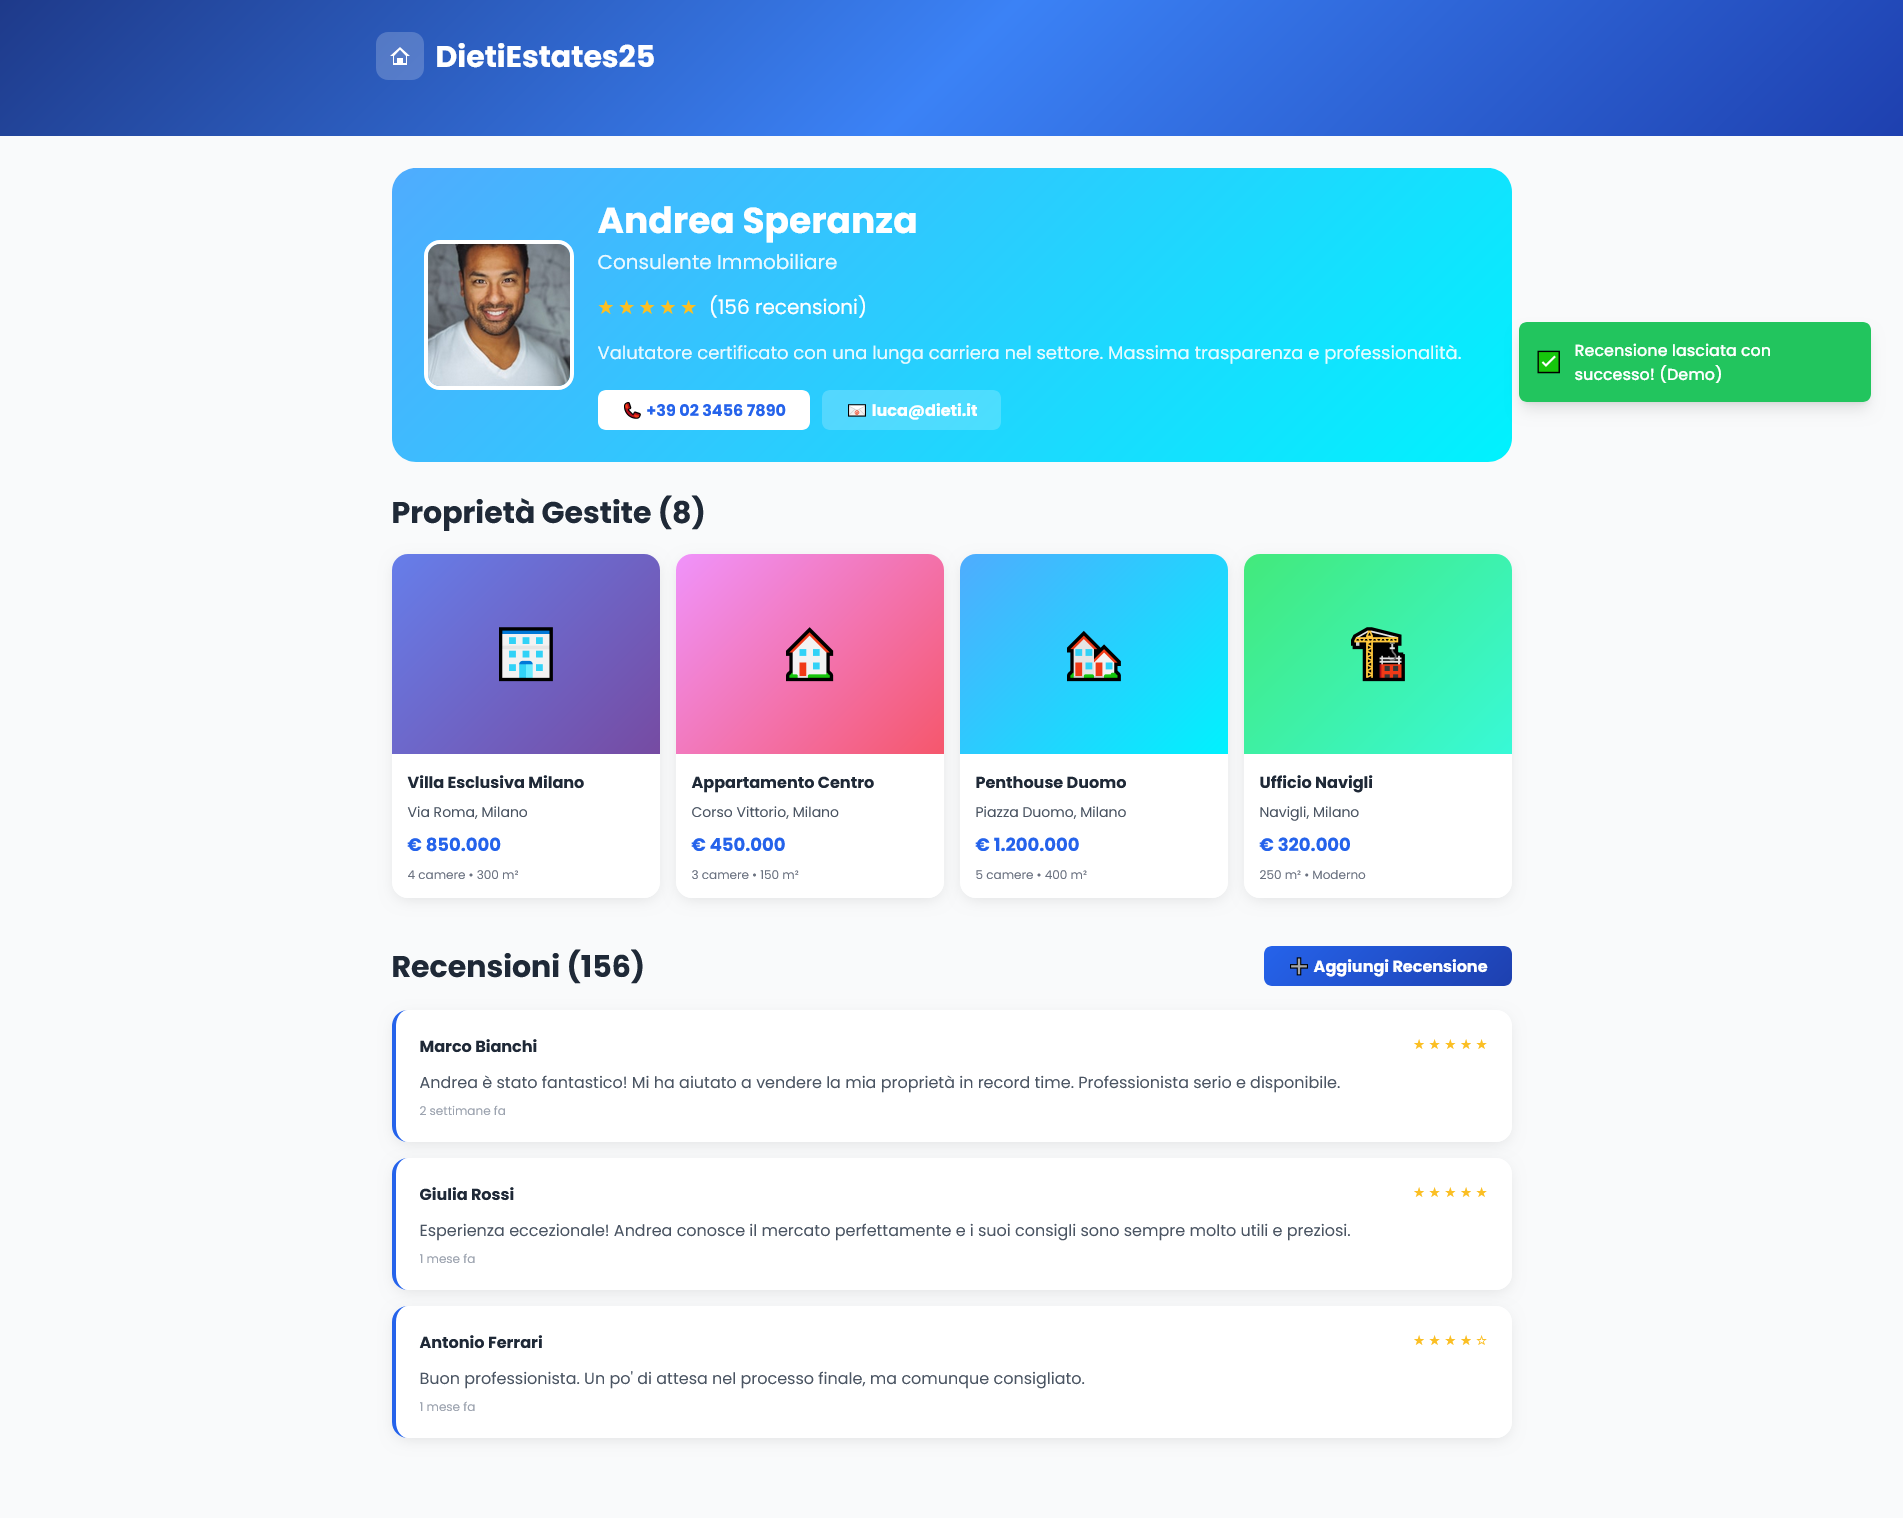
\includegraphics[width=\textwidth]{pics/ReviewSuccess.png}
    \caption{Recensione Aggiunta}
\end{figure}

\pagebreak

\section{Formalizzazione di casi d’uso (Cockburn)}
Di seguito quattro casi d’uso significativi (esclusi quelli di registrazione/autenticazione), formalizzati secondo Cockburn.

\subsection*{UC06 -- Ricerca avanzata di immobili}

\begin{table}[H]
\centering
\small
\setlength{\tabcolsep}{3pt} % Ridotto leggermente per far stare le 4 colonne
\renewcommand{\arraystretch}{1.3}
\noindent
\begin{tabularx}{\linewidth}{|p{3cm}|c|X|X|}
\hline
\textbf{USE CASE \#06} & \multicolumn{3}{l|}{\textbf{Ricerca avanzata immobili}} \\ \hline
\textbf{Goal in Context} & \multicolumn{3}{l|}{Trovare immobili con filtri e mappa.} \\ \hline
\textbf{Preconditions} & \multicolumn{3}{l|}{DB popolato, servizi attivi.} \\ \hline
\textbf{Success End Cond.} & \multicolumn{3}{l|}{Lista immobili e marker su mappa visualizzati.} \\ \hline
\textbf{Failed End Cond.} & \multicolumn{3}{l|}{Nessun immobile trovato.} \\ \hline
\textbf{Primary Actor} & \multicolumn{3}{l|}{Utente (Visitatore/Cliente)} \\ \hline
\textbf{Trigger} & \multicolumn{3}{l|}{Click su "Properties" nella Navbar.} \\ \hline
\textbf{Main Scenario} & \textbf{Step} & \textbf{Actor Action} & \textbf{System Action} \\ \hline 
 & 1 & Va su \textbf{M1} e preme "Properties". &  \\ \cline{2-4} 
 & 2 & & Mostra \textbf{M2} (Ricerca) con filtri default. \\ \cline{2-4} 
 & 3 & Imposta filtri e preme "Cerca". &  \\ \cline{2-4} 
 & 4 & & Mostra risultati su lista e mappa in \textbf{M2}. \\ \hline
\textbf{Extensions} & \textbf{Step} & \textbf{Condition} & \textbf{System Action} \\ \hline 
 & 4a & Nessun risultato trovato. & Mostra \textbf{M3} (Ricerca Senza Risultati). \\ \hline
\end{tabularx}
\caption{UC06 - Ricerca Immobili}
\end{table}


\pagebreak

\subsection*{UC08 -- Creazione di un nuovo immobile (agente)}

\begin{table}[ht]
\centering
\small
\setlength{\tabcolsep}{3pt}
\renewcommand{\arraystretch}{1.3}
\noindent
\begin{tabularx}{\linewidth}{|p{3cm}|c|X|X|}
\hline
\textbf{USE CASE \#08} & \multicolumn{3}{l|}{\textbf{Creazione annuncio immobile}} \\ \hline
\textbf{Goal in Context} & \multicolumn{3}{l|}{Agente pubblica nuovo immobile.} \\ \hline
\textbf{Preconditions} & \multicolumn{3}{l|}{Login effettuato come Agente.} \\ \hline
\textbf{Success End Cond.} & \multicolumn{3}{l|}{Immobile salvato e visibile.} \\ \hline
\textbf{Failed End Cond.} & \multicolumn{3}{l|}{Salvataggio fallito (dati incompleti).} \\ \hline
\textbf{Primary Actor} & \multicolumn{3}{l|}{Agente Immobiliare} \\ \hline
\textbf{Trigger} & \multicolumn{3}{l|}{Click su "Dashboard" nella Navbar.} \\ \hline
\textbf{Main Scenario} & \textbf{Step} & \textbf{Actor Action} & \textbf{System Action} \\ \hline 
 & 1 & Dalla \textbf{M1}, va alla Dashboard. & Mostra \textbf{M4} (Dashboard). \\ \cline{2-4} 
 & 2 & Preme "Aggiungi Proprietà". & Mostra \textbf{M5} (Creazione). \\ \cline{2-4} 
 & 3 & Compila campi e preme "Salva". &  \\ \cline{2-4} 
 & 4 & & Valida e salva. Mostra \textbf{M4} aggiornata. \\ \hline
\textbf{Extensions} & \textbf{Step} & \textbf{Condition} & \textbf{System Action} \\ \hline 
 & 3a & Campi obbligatori vuoti. & Mostra \textbf{M6} (Campi Incompleti) ed errori. \\ \hline
\end{tabularx}
\caption{UC08 - Creazione Immobile}
\end{table}

\pagebreak

\subsection*{UC10 -- Gestione profilo agente (biografia e foto)}

\begin{table}[ht]
\centering
\small
\setlength{\tabcolsep}{3pt}
\renewcommand{\arraystretch}{1.3}
\noindent
\begin{tabularx}{\linewidth}{|p{3cm}|c|X|X|}
\hline
\textbf{USE CASE \#10} & \multicolumn{3}{l|}{\textbf{Gestione profilo agente}} \\ \hline
\textbf{Goal in Context} & \multicolumn{3}{l|}{Aggiornamento dati e biografia.} \\ \hline
\textbf{Preconditions} & \multicolumn{3}{l|}{Login effettuato come Agente.} \\ \hline
\textbf{Success End Cond.} & \multicolumn{3}{l|}{Dati aggiornati a sistema.} \\ \hline
\textbf{Failed End Cond.} & \multicolumn{3}{l|}{Modifiche non salvate.} \\ \hline
\textbf{Primary Actor} & \multicolumn{3}{l|}{Agente Immobiliare} \\ \hline
\textbf{Trigger} & \multicolumn{3}{l|}{Click su "Profilo" nella Navbar.} \\ \hline
\textbf{Main Scenario} & \textbf{Step} & \textbf{Actor Action} & \textbf{System Action} \\ \hline 
 & 1 & Preme "Profilo". & Mostra \textbf{M7} (Profilo). \\ \cline{2-4} 
 & 2 & Preme "Modifica". & Mostra \textbf{M8} (Modifica in Corso). \\ \cline{2-4} 
 & 3 & Modifica dati e preme "Salva". &  \\ \cline{2-4} 
 & 4 & & Salva e mostra \textbf{M9} (Successo). \\ \hline
\textbf{Extensions} & \multicolumn{3}{c|}{(Nessuna estensione critica prevista)} \\ \hline
\end{tabularx}
\caption{UC10 - Gestione Profilo}
\end{table}

\pagebreak

\subsection*{UC12 -- Inserimento recensione agente}

\begin{table}[ht]
\centering
\small
\setlength{\tabcolsep}{3pt}
\renewcommand{\arraystretch}{1.3}
\noindent
\begin{tabularx}{\linewidth}{|p{3cm}|c|X|X|}
\hline
\textbf{USE CASE \#12} & \multicolumn{3}{l|}{\textbf{Inserimento recensione agente}} \\ \hline
\textbf{Goal in Context} & \multicolumn{3}{l|}{Valutare agente con voto e testo.} \\ \hline
\textbf{Preconditions} & \multicolumn{3}{l|}{Utente loggato.} \\ \hline
\textbf{Success End Cond.} & \multicolumn{3}{l|}{Recensione salvata.} \\ \hline
\textbf{Failed End Cond.} & \multicolumn{3}{l|}{Recensione non inviata.} \\ \hline
\textbf{Primary Actor} & \multicolumn{3}{l|}{Utente Registrato} \\ \hline
\textbf{Trigger} & \multicolumn{3}{l|}{Selezione agente dalla lista.} \\ \hline
\textbf{Main Scenario} & \textbf{Step} & \textbf{Actor Action} & \textbf{System Action} \\ \hline 
 & 1 & Seleziona un agente. & Mostra \textbf{M10} (Dettaglio Agente). \\ \cline{2-4} 
 & 2 & Preme "Aggiungi Recensione". & Mostra form \textbf{M11}. \\ \cline{2-4} 
 & 3 & Inserisce dati e preme "Invia". &  \\ \cline{2-4} 
 & 4 & & Registra e mostra \textbf{M12} (Review Aggiunta). \\ \hline
\textbf{Extensions} & \multicolumn{3}{c|}{(Nessuna estensione critica prevista)} \\ \hline
\end{tabularx}
\caption{UC12 - Inserimento Recensione}
\end{table}

\pagebreak

\clearpage
\chapter{Documento di Design del sistema}

\section{Architettura}

L’architettura globale è di tipo client-server:

\begin{itemize}[nosep]
  \item \textbf{Front-end:} Single Page Application Angular 21.
  \item \textbf{Back-end:} REST API Spring Boot 3.2.
  \item \textbf{Database:} H2 in sviluppo (modalità PostgreSQL), PostgreSQL/PostGIS in produzione.
  \item \textbf{Storage file:} AWS S3 (o storage locale) incapsulato in un servizio di storage.
  \item \textbf{Autenticazione:} JWT per le API; OAuth2 per login sociale.
\end{itemize}

\subsection{Strati logici back-end}

Il back-end adotta una architettura \textbf{a tre livelli} (Controller--Service--Repository), tipica dei sistemi enterprise basati su Spring. Questo pattern separa nettamente:

\begin{itemize}[nosep]
  \item la gestione delle richieste HTTP,
  \item la logica di dominio e di business,
  \item l'accesso ai dati persistenti.
\end{itemize}

In dettaglio:

\begin{itemize}[nosep]
    \item \textbf{Presentation layer (Controller)}:
    \begin{itemize}[nosep]
      \item espone endpoint REST e mappa le richieste HTTP verso operazioni di business;
      \item valida i dati di input a livello di request (es. annotazioni \texttt{@Valid} su DTO di ingresso);
      \item traduce le entità/DTO interni in risposte HTTP (codici di stato, payload JSON).
    \end{itemize}
    
    \item \textbf{Business layer (Service)}:
    \begin{itemize}[nosep]
      \item contiene la logica di dominio (es. regole di creazione immobili, associazione ad agenti e agenzie, calcolo e aggregazione delle recensioni);
      \item coordina l'accesso ai repository e ad altri servizi (es. \texttt{StorageService}, \texttt{JwtService}, servizi di notifica);
      \item rappresenta il \emph{punto di ingresso} per i casi d'uso applicativi (UC06, UC08, UC10, UC12), rendendo più semplice il testing unitario delle regole di business.
    \end{itemize}
\end{itemize}

\pagebreak

    \subsection{Pattern architetturali e di design}
    
    Nell'implementazione di DietiEstates25 sono stati applicati diversi pattern architetturali e di design:
    
\begin{itemize}    
    \item \textbf{Layered Architecture}:
    l'organizzazione in livelli Controller--Service--Repository segue un'architettura stratificata, che separa presentazione, logica di business e accesso ai dati.
    
    \item \textbf{Repository Pattern}:
    le interfacce \texttt{*Repository} incapsulano le operazioni di persistenza sulle entità di dominio, fornendo un'API ad alto livello indipendente dal database sottostante (H2 in sviluppo, PostgreSQL/PostGIS in produzione).
    
    \item \textbf{DTO (Data Transfer Object)}:
    l'uso di \texttt{*DTO} per richieste e risposte REST separa il modello interno dal contratto esterno delle API, riducendo il coupling e facilitando l'evoluzione del dominio e della versione delle API.
    
    \item \textbf{Dependency Injection / Inversion of Control}:
    i componenti Spring (controller, servizi, repository) e i servizi Angular sono istanziati e collegati dal container IoC, migliorando testabilità e sostituibilità delle dipendenze (ad esempio, \texttt{StorageService} può essere sostituito con uno stub per i test). 
    
    Questi pattern supportano gli obiettivi di \textbf{manutenibilità}, \textbf{riusabilità} e \textbf{scalabilità} definiti nei requisiti non funzionali, e rendono l'architettura coerente con le best practice dei framework utilizzati (Spring Boot e Angular).
    
    \item \textbf{Data access layer (Repository)}:
    \begin{itemize}[nosep]
      \item astrae le operazioni CRUD sul database tramite Spring Data JPA;
      \item definisce metodi di query ad alto livello (es. \texttt{findByCityAndPriceBetween(...)} o query personalizzate per la ricerca geografica);
      \item isola il resto dell'applicazione dai dettagli del database (PostgreSQL/H2, PostGIS).
    \end{itemize}
\end{itemize}
Questa suddivisione:

\begin{itemize}[nosep]
  \item migliora la \textbf{manutenibilità} (i cambiamenti in un livello impattano minimamente sugli altri);
  \item favorisce la \textbf{testabilità} (i service possono essere testati isolando i repository tramite mock);
  \item rende l'architettura \textbf{estendibile}, permettendo l'aggiunta di nuovi use case o integrazioni senza modificare i controller esistenti.
\end{itemize}

\subsection{Struttura front-end}

\begin{itemize}[nosep]
  \item Cartella \texttt{features/}:
    \begin{itemize}[nosep]
      \item \texttt{auth}: login, registrazione.
      \item \texttt{properties}: lista, dettaglio, creazione.
      \item \texttt{agents}: lista, dettaglio, dashboard agente.
      \item \texttt{agency}: dashboard manager e creazione agenti.
      \item \texttt{profile}: gestione profilo utente/agente.
      \item \texttt{home}: pagina principale con ricerca.
    \end{itemize}
  \item Cartella \texttt{core/}: servizi, modelli, interceptor JWT.
  \item Cartella \texttt{shared/}: componenti riutilizzabili (navbar, property-card, map-search, dual-range-slider, toast, footer).
\end{itemize}

\section{Criteri di design}

\begin{itemize}[nosep]
  \item \textbf{Separation of Concerns:} controller sottili, logica concentrata nei servizi.
  \item \textbf{DTO e Request objects:} per separare il modello interno dal contratto esterno delle API.
  \item \textbf{Security by design:} filtri JWT, configurazione fine-grained di ruoli e permessi.
  \item \textbf{Configurazione esterna:} parametri sensibili (JWT secret, chiavi OAuth, AWS) in variabili d’ambiente.
  \item \textbf{Estendibilità:} uso di enum e astrazioni di servizio per supportare facilmente nuove tipologie e provider.
\end{itemize}

\section{Tecnologie adottate}

\subsection{Back-end}

\begin{itemize}[nosep]
  \item \textbf{Spring Boot 3.2.1} (web, data-jpa, validation, security, oauth2-client).
  \item \textbf{Hibernate + Hibernate Spatial} per persistenza e tipi spaziali.
  \item \textbf{Spring Security + JWT} per autenticazione stateless.
  \item \textbf{H2} in-memory per sviluppo; \textbf{PostgreSQL/PostGIS} per produzione.
  \item \textbf{Lombok} per ridurre boilerplate.
  \item \textbf{SpringDoc OpenAPI} per documentazione API (Swagger UI).
\end{itemize}

\subsection{Front-end}

\begin{itemize}[nosep]
  \item \textbf{Angular 21} con standalone components.
  \item \textbf{@angular/google-maps} per integrazione mappa.
  \item \textbf{RxJS} per la gestione asincrona.
  \item \textbf{Vitest} per unit test.
\end{itemize}

\subsection{DevOps e strumenti}

\begin{itemize}[nosep]
  \item \textbf{Maven} per build e gestione dipendenze.
  \item \textbf{Docker} per containerizzazione.
  \item \textbf{JaCoCo} per coverage.
  \item \textbf{SonarQube} per analisi qualità del codice back-end.
\end{itemize}

\pagebreak

\section{Deployment e infrastruttura}

Il sistema è pensato per un deployment su infrastruttura cloud, con particolare riferimento ad \textbf{AWS}.

\subsection{Back-end e database}

Il back-end \textbf{Spring Boot} è eseguito su una \textbf{Virtual Machine AWS} (es. istanza EC2) che ospita anche il database \textbf{PostgreSQL/PostGIS} utilizzato in produzione. In questo scenario:

\begin{itemize}[nosep]
  \item l'applicazione Spring Boot è deployata come \texttt{jar} eseguibile (o container Docker) sulla VM;
  \item PostgreSQL/PostGIS è installato e configurato sulla stessa VM, con accesso limitato tramite regole di sicurezza (security group, firewall);
  \item l'applicazione accede al database tramite credenziali configurate in variabili d'ambiente o file di configurazione esterni.
\end{itemize}

Questa configurazione semplifica la gestione iniziale dell'infrastruttura, mantenendo comunque la possibilità di evolvere verso una separazione tra application server e database server o verso servizi gestiti (ad es. Amazon RDS) in fasi successive.

\subsection{Storage delle immagini}

Le immagini (foto immobili e foto profilo agenti) non risiedono sulla VM, ma sono caricate in un \textbf{bucket Amazon S3} dedicato. L'applicazione:

\begin{itemize}[nosep]
  \item riceve i file dal front-end tramite endpoint REST;
  \item li inoltra al bucket S3 tramite \texttt{StorageService}, che incapsula le API AWS;
  \item memorizza nel database solo i riferimenti (URL e metadati), mantenendo il back-end stateless rispetto ai contenuti binari.
\end{itemize}

Questo approccio consente di:

\begin{itemize}[nosep]
  \item ridurre il carico di I/O sulla VM;
  \item scalare indipendentemente l'application server e lo storage;
  \item semplificare il backup e la replica dei contenuti multimediali.
\end{itemize}

\pagebreak

\section{Schema di persistenza dati}

Dal punto di vista infrastrutturale, la persistenza dei dati è articolata su due piani principali:

\begin{itemize}[nosep]
  \item \textbf{Dati applicativi strutturati} (utenti, agenzie, immobili, recensioni, ecc.) memorizzati in un database relazionale.
  \item \textbf{Contenuti multimediali} (foto degli immobili, foto profilo agenti) memorizzati come file in uno storage oggetti esterno.
\end{itemize}

In ambiente di sviluppo viene utilizzato \textbf{H2} in-memory in modalità PostgreSQL per velocizzare il ciclo di sviluppo e testing, mentre in produzione i dati sono persistiti in un database \textbf{PostgreSQL/PostGIS} eseguito su una \textbf{Virtual Machine AWS} dedicata. Il back-end Spring Boot si connette a tale istanza tramite JDBC, sfruttando PostGIS per la gestione delle coordinate geografiche (ricerca per raggio, visualizzazione su mappa).

Le foto degli immobili e le immagini di profilo non sono salvate direttamente nel database, ma in un \textbf{bucket S3} dedicato. Il back-end interagisce con S3 tramite un componente \texttt{StorageService} che incapsula:

\begin{itemize}[nosep]
  \item il caricamento dei file (upload) verso il bucket;
  \item la generazione e gestione degli URL pubblici o firmati;
  \item l’eventuale cancellazione o aggiornamento delle immagini.
\end{itemize}

Nel database vengono quindi memorizzati solo i \textbf{metadati} (es. URL, nome file, ordine nella galleria) necessari a collegare ciascun record applicativo al corrispondente file nel bucket S3. In questo modo:

\begin{itemize}[nosep]
  \item si mantiene il database snello e performante;
  \item si delega la scalabilità e l’affidabilità dello storage dei file a S3;
  \item si semplifica il deploy del back-end, che resta stateless rispetto ai contenuti multimediali.
\end{itemize}

A livello di modello concettuale, le principali entità sono:

\begin{itemize}[nosep]
  \item \textbf{User}:
    \begin{itemize}[nosep]
      \item Attributi: \texttt{id}, \texttt{email}, \texttt{password\_hash}, \texttt{first\_name}, \texttt{last\_name}, \texttt{registered\_at}, \texttt{is\_active}, \texttt{auth\_provider}.
      \item Relazioni: molti-a-uno con \texttt{Agency}; molti-a-molti con \texttt{Role}.
    \end{itemize}
  \item \textbf{Agent} (sottoclasse di \texttt{User}):
    \begin{itemize}[nosep]
      \item Attributi addizionali: biografia, foto profilo (URL S3), data di nascita, numero di telefono.
    \end{itemize}
  \item \textbf{Agency}:
    \begin{itemize}[nosep]
      \item Attributi: \texttt{id}, \texttt{name}, \texttt{email}, \texttt{phone}, \texttt{address}, \texttt{created\_at}.
      \item Relazioni: uno-a-molti con utenti/agent; uno-a-molti con property.
    \end{itemize}
  \item \textbf{Property}:
    \begin{itemize}[nosep]
      \item Attributi: titolo, descrizione, prezzo, tipo (SALE/RENT), metratura, stanze, piano, bagni, condizione, anno, classe energetica, indirizzo, città, posizione geografica (tipo spaziale PostGIS).
      \item Relazioni: molti-a-uno con \texttt{Agent} e \texttt{Agency}; uno-a-molti con \texttt{PropertyPhoto}; molti-a-molti con \texttt{Amenity}.
    \end{itemize}
  \item \textbf{Amenity}: \texttt{id}, \texttt{name} (univoco), relazione molti-a-molti con property.
  \item \textbf{PropertyPhoto}: \texttt{id}, \texttt{url} (verso S3), eventuali metadati (ordine, descrizione), FK a property.
  \item \textbf{Review}: \texttt{id}, \texttt{score}, \texttt{comment}, \texttt{created\_at}, FK a \texttt{Agent} e \texttt{User}.
\end{itemize}



\section{Design dell’interfaccia utente}

Principi generali:

\begin{itemize}[nosep]
  \item \textbf{Navigazione chiara:} navbar fissa con accesso a Home, Properties, Agents, Profile/Login.
  \item \textbf{Home page:} sezione \emph{hero} con testo introduttivo e box di ricerca rapida.
  \item \textbf{Ricerca/listing:} form filtri in alto, lista di immobili in card e mappa affiancata.
  \item \textbf{Dettaglio immobile:} galleria foto, dati essenziali, mappa, contatti agente/agenzia.
  \item \textbf{Login/Registrazione:} layout a due colonne (branding + form), pulsanti social login, messaggi di validazione chiari.
  \item \textbf{Profilo utente/agente:} pagina con card dati personali e, per agenti, colonna dedicata a foto/biografia.
\end{itemize}

\pagebreak
\section{Diagramma delle classi di design}

Il diagramma delle classi di design rappresenta:

\begin{itemize}[nosep]
  \item Gerarchia utenti: \texttt{User} e sottoclasse \texttt{Agent}.
  \item Dominio immobiliare: \texttt{Property}, \texttt{Agency}, \texttt{Amenity}, \texttt{PropertyPhoto}, \texttt{Review}.
  \item Relazioni tra servizi e repository: \texttt{PropertyService}, \texttt{AgentService}, \texttt{AuthService} con i rispettivi \texttt{*Repository}.
\end{itemize}

\begin{figure}[H]
    \centering
    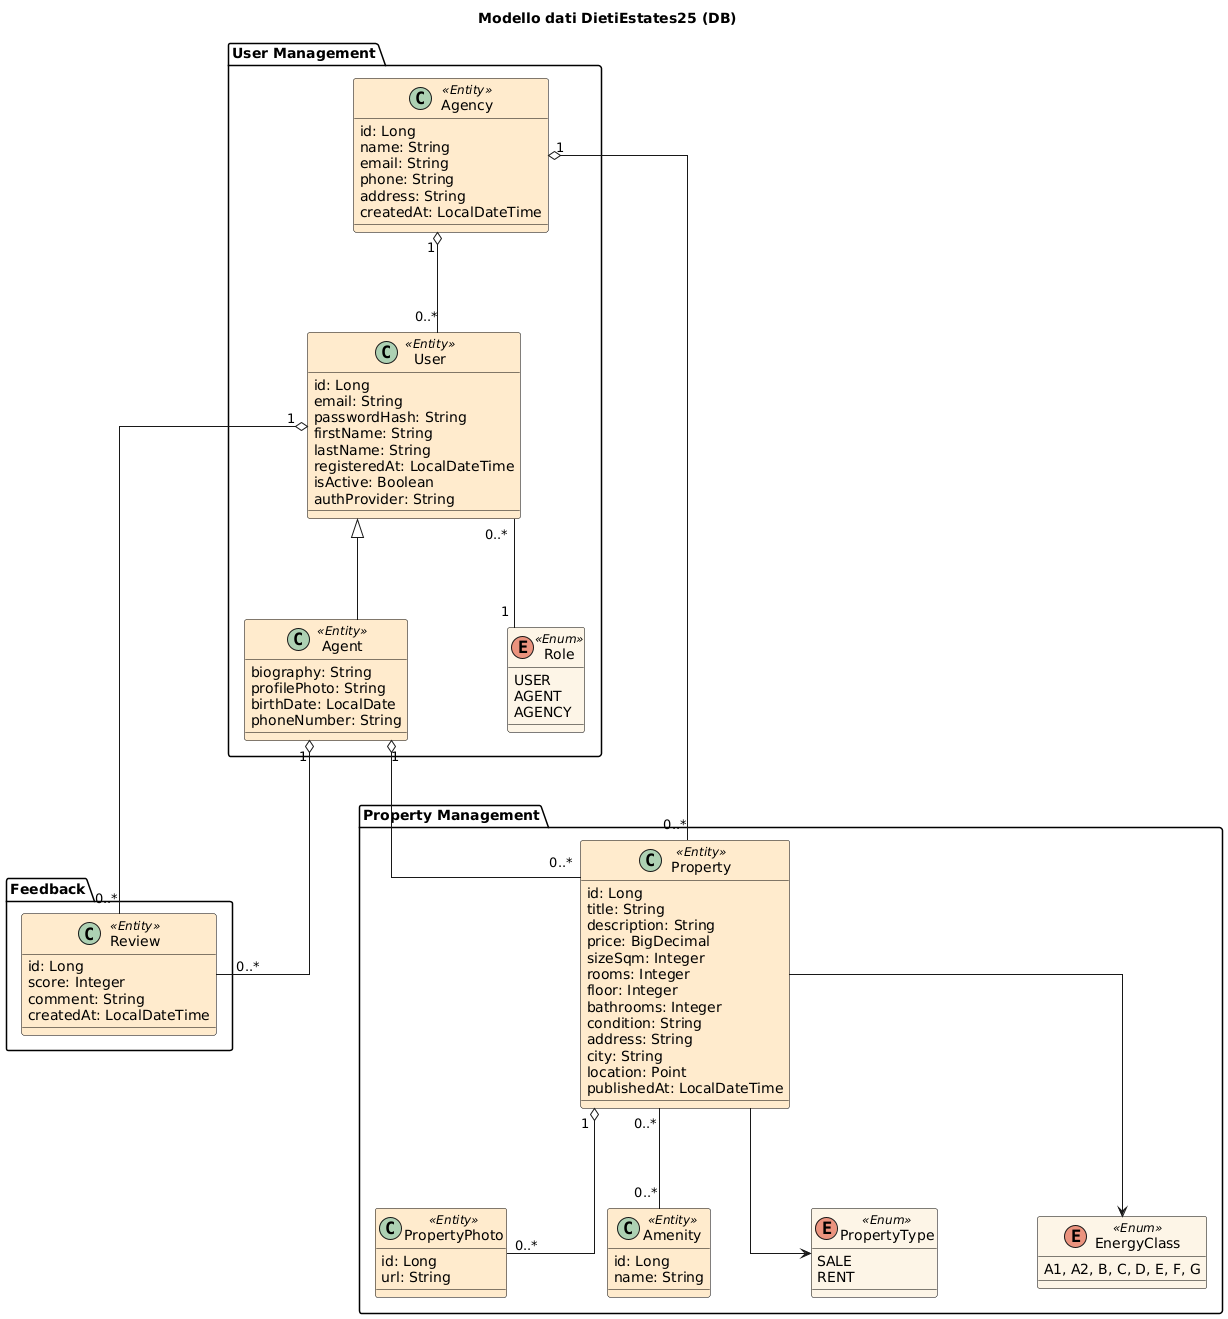
\includegraphics[width=\textwidth]{pics/DB.png}
    \caption{Diagramma delle classi di Design}
\end{figure}

\subsection{Diagrammi Architetturali}

Di seguito viene rappresentata l'architettura del BackEnd con diagrammi di dettaglio per il pacchetto Controller e Service.

\begin{figure}[H]
    \centering
    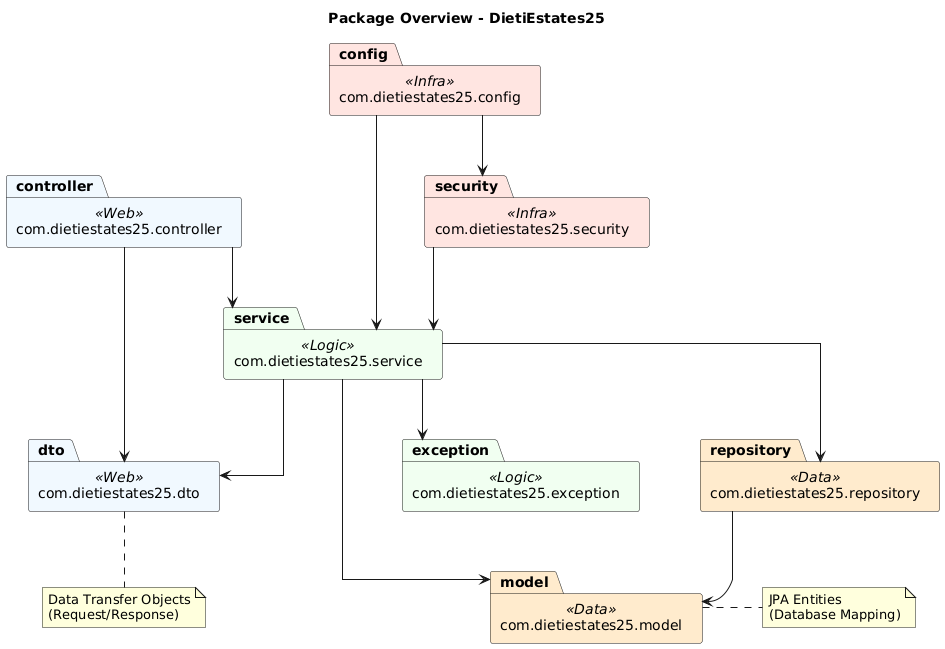
\includegraphics[width=\textwidth]{pics/PackageOverview.png}
    \caption{System Overview}
\end{figure}

\pagebreak

\begin{figure}[H]
    \centering
    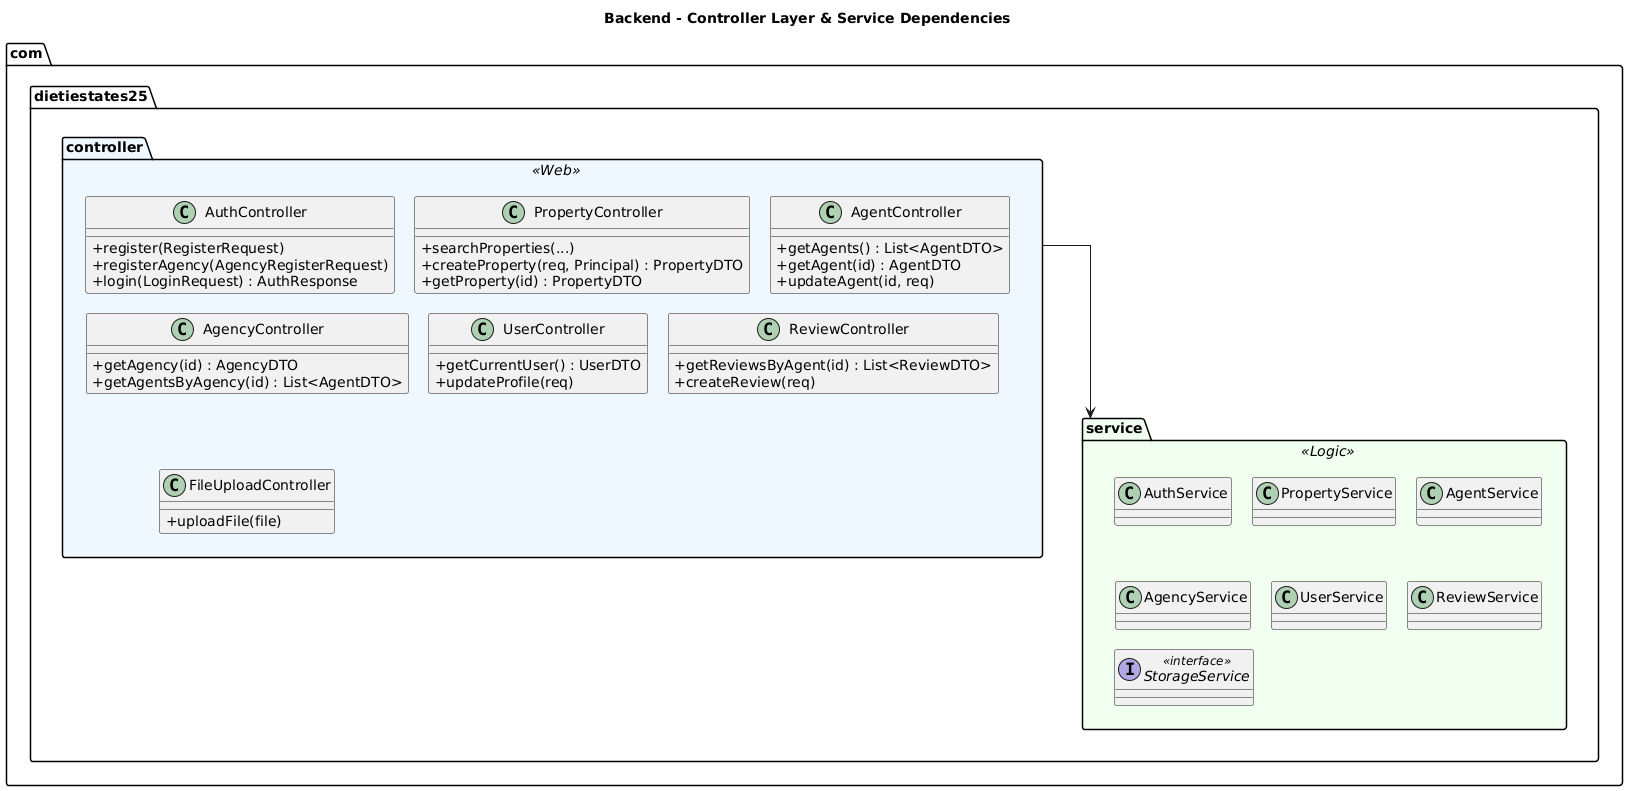
\includegraphics[width=\textwidth]{pics/Controller.png}
    \caption{Detailed Controller View}
\end{figure}

\begin{figure}[H]
    \centering
    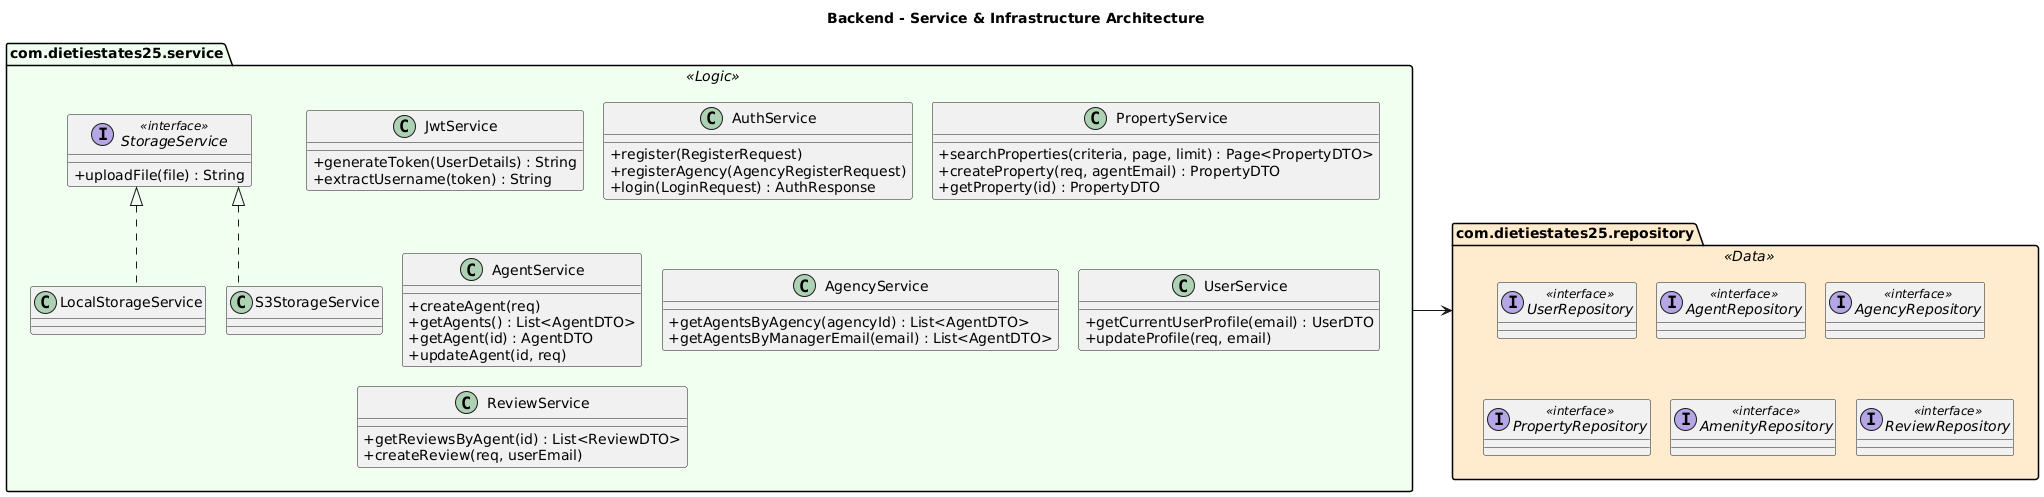
\includegraphics[width=\textwidth]{pics/Service.png}
    \caption{Detailed Service View}
\end{figure}

\pagebreak

\section{Diagrammi di sequenza}

Per i casi d’uso UC06, UC08, UC10 e UC12 sono definiti i seguenti diagrammi di sequenza.

\subsection{Sequence Diagram: UC06}

\begin{figure}[H]
    \centering
    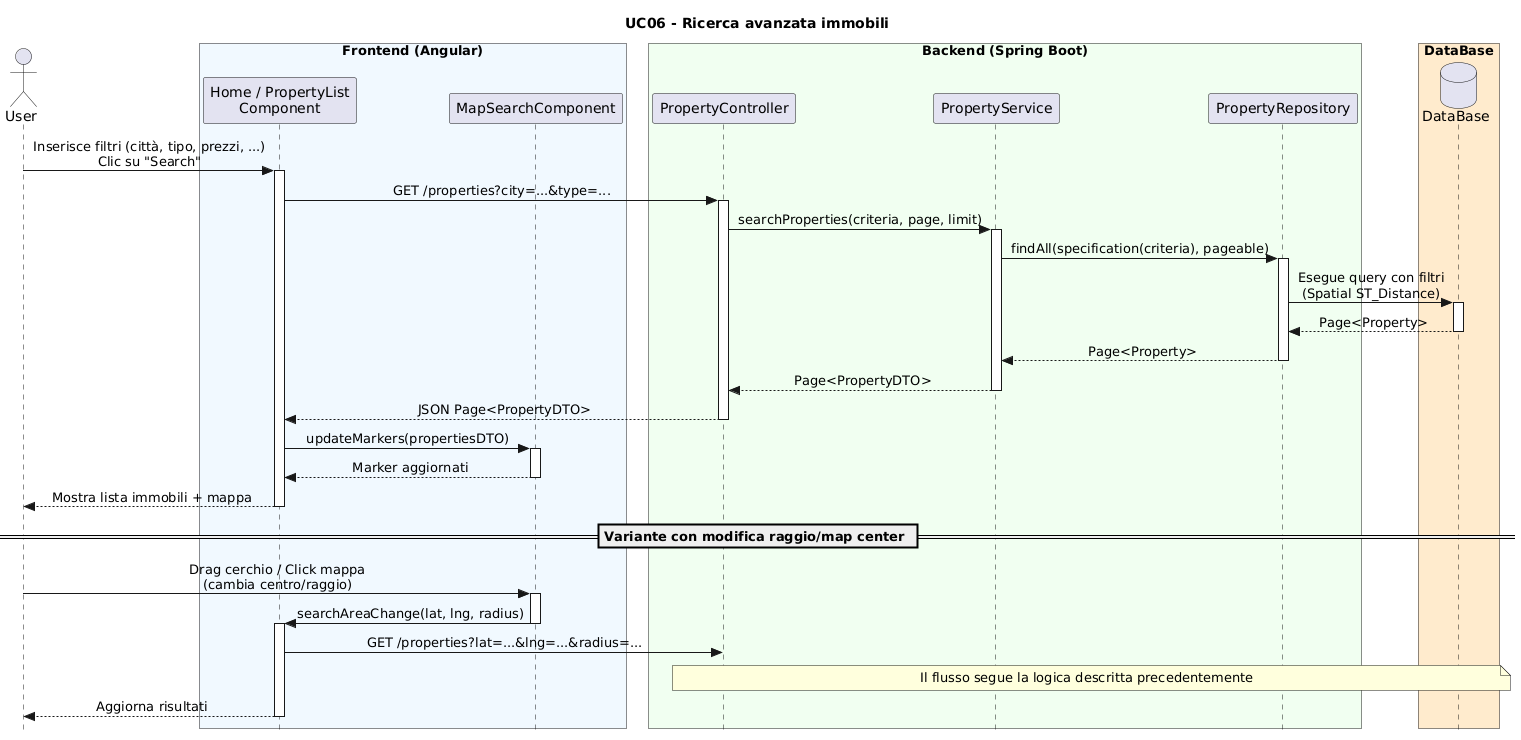
\includegraphics[width=\textwidth]{pics/UC06.png}
    \caption{Sequence Diagram: UC06}
\end{figure}

\subsection{Sequence Diagram: UC08}

\begin{figure}[H]
    \centering
    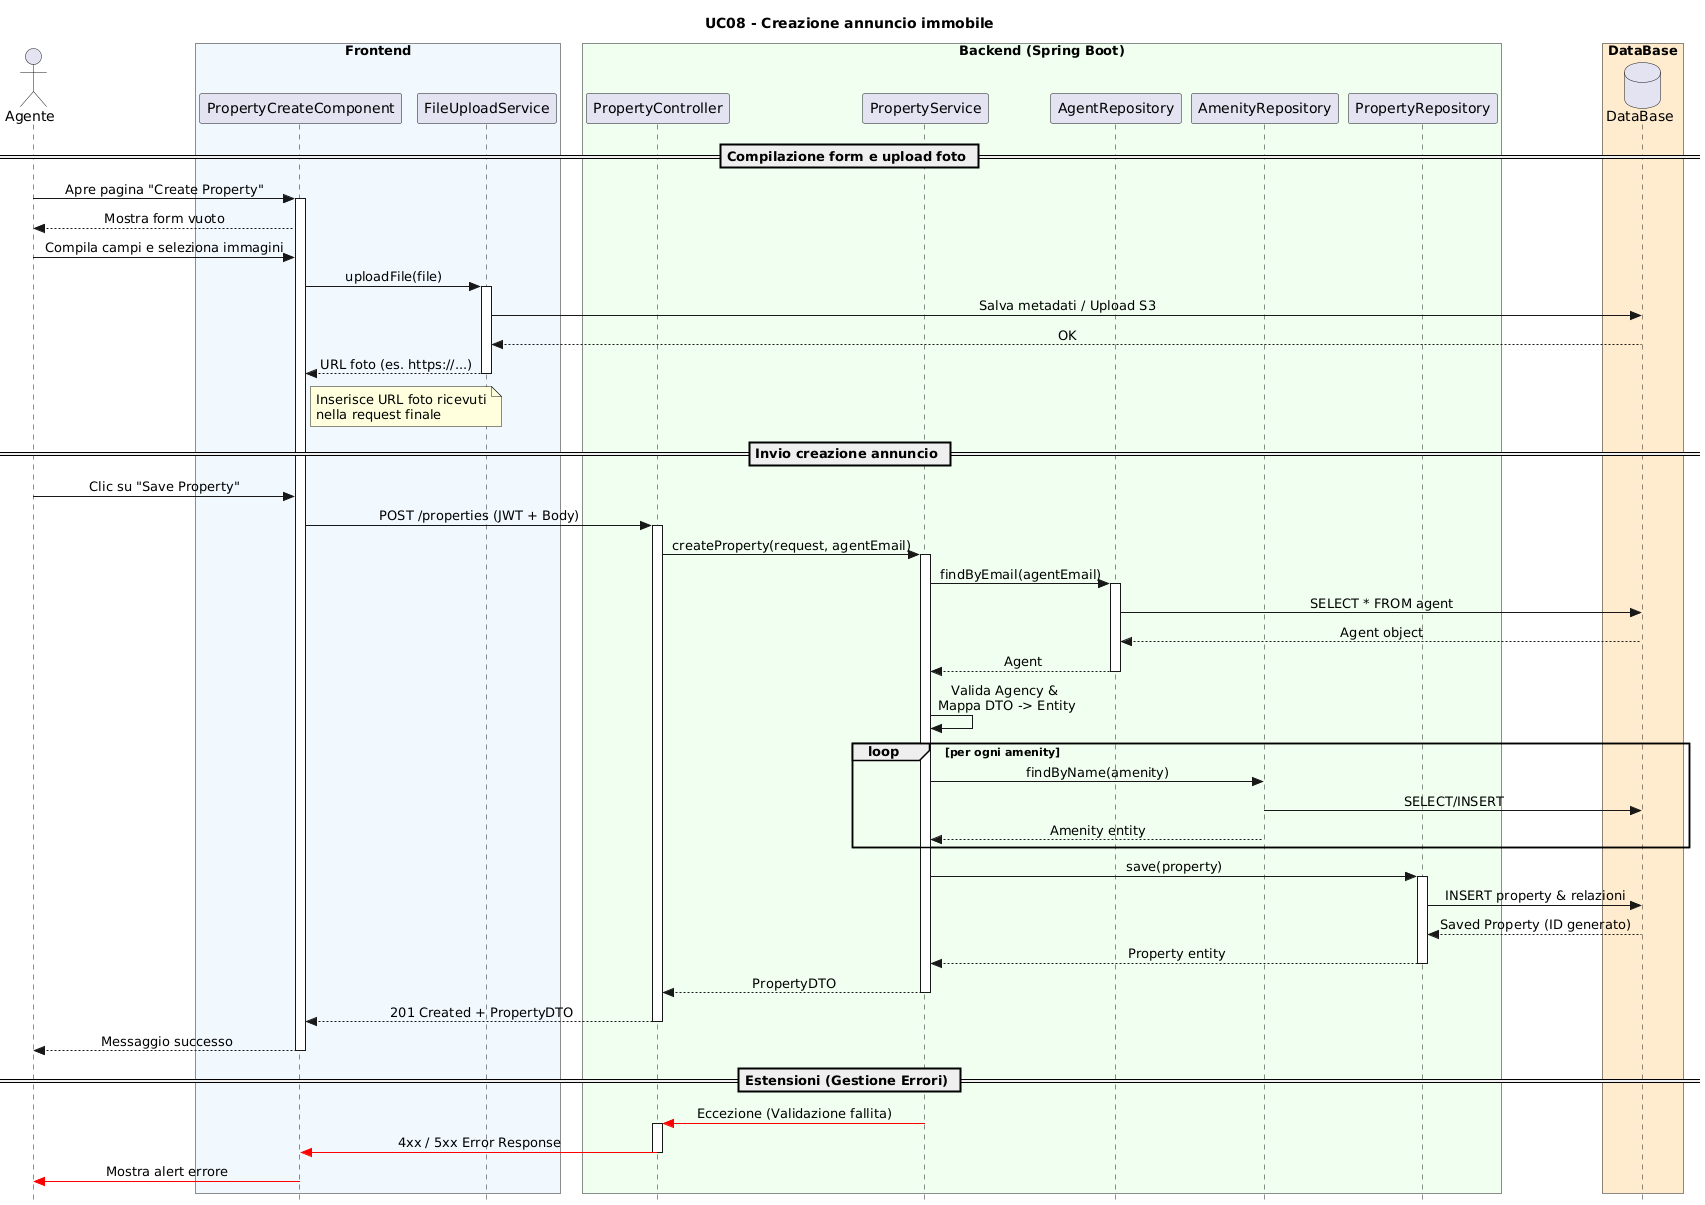
\includegraphics[width=\textwidth]{pics/UC08.png}
    \caption{Sequence Diagram: UC08}
\end{figure}

\subsection{Sequence Diagram: UC10}

\begin{figure}[H]
    \centering
    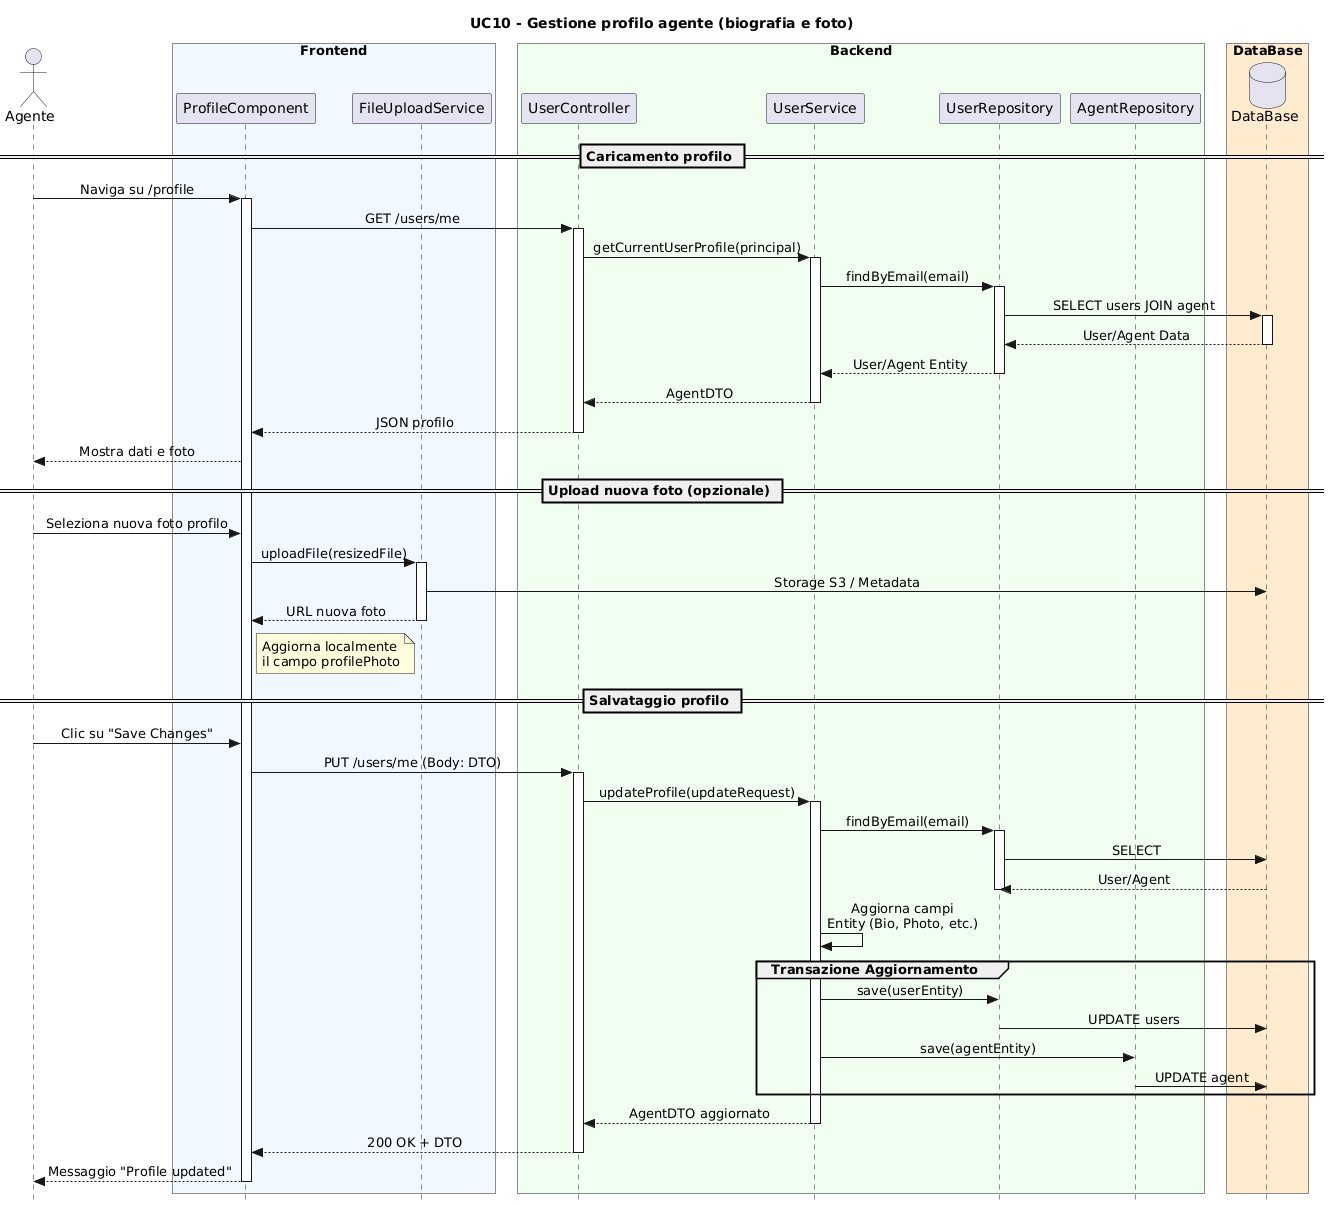
\includegraphics[width=\textwidth]{pics/UC10.png}
    \caption{Sequence Diagram: UC10}
\end{figure}

\subsection{Sequence Diagram: UC12}

\begin{figure}[H]
    \centering
    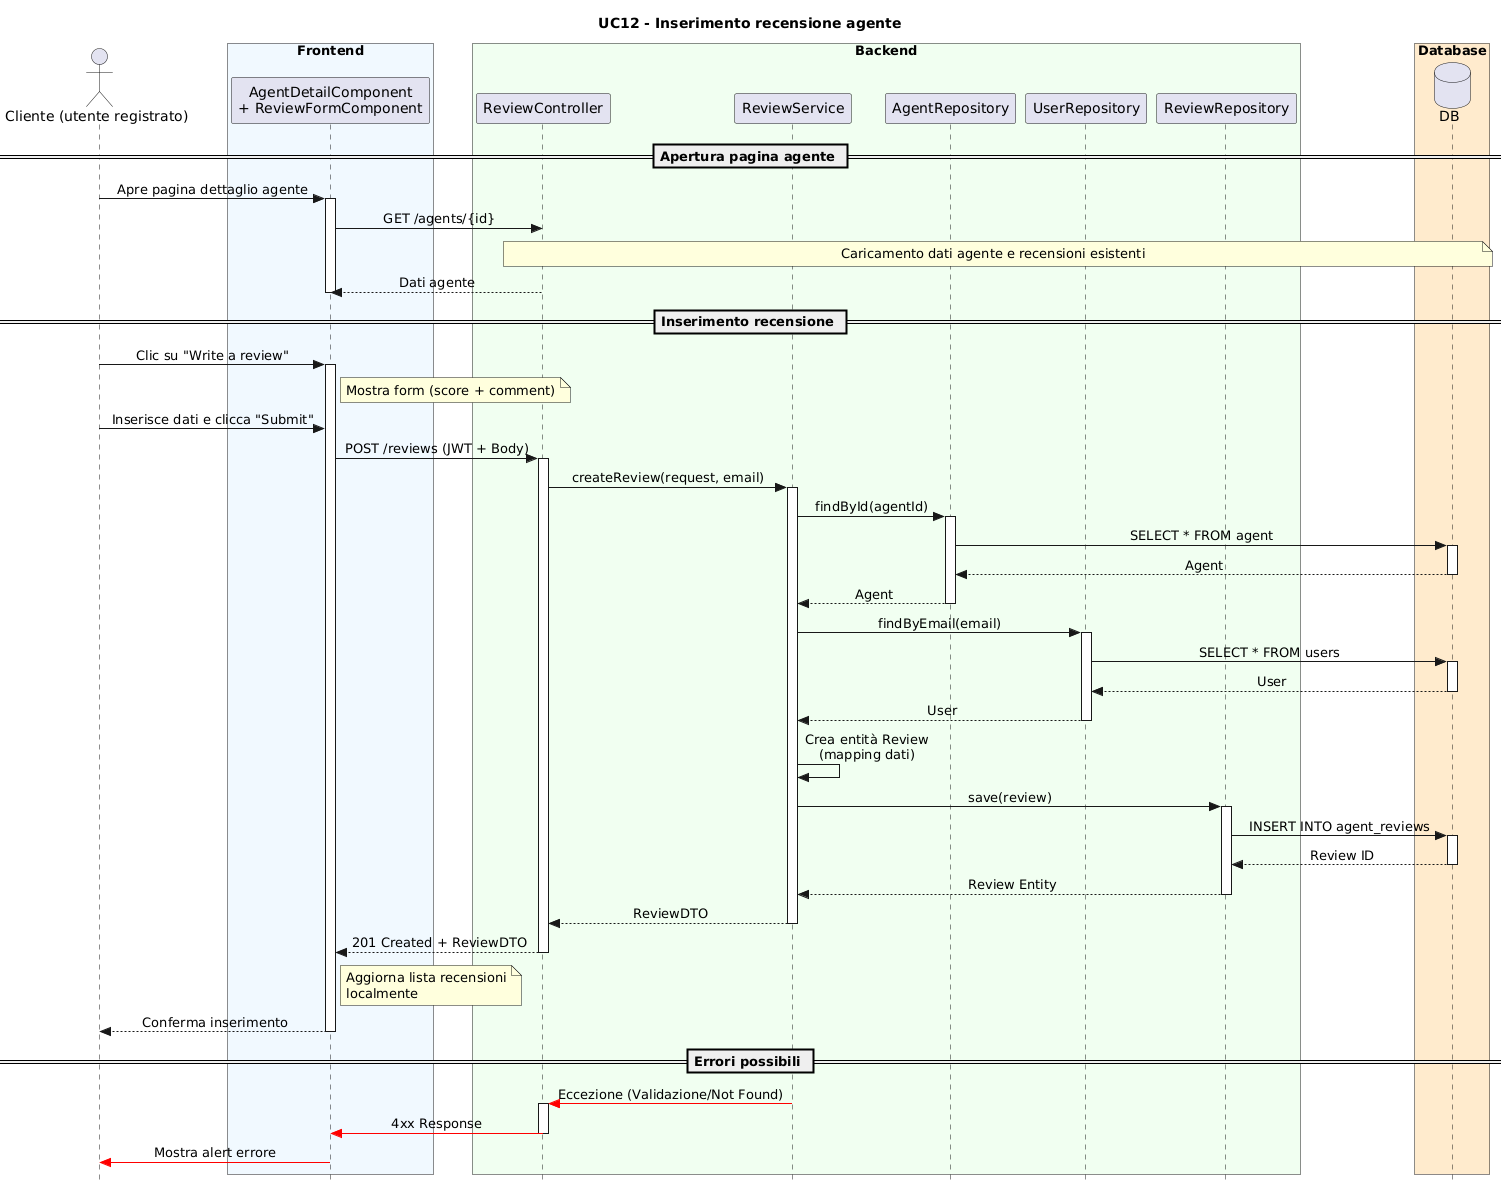
\includegraphics[width=\textwidth]{pics/UC12.png}
    \caption{Sequence Diagram: UC12}
\end{figure}


\clearpage

\section{Gestione del versioning}

Il progetto utilizza \textbf{Git} come sistema di versioning distribuito, con repository ospitato su \textbf{GitHub}. Questa scelta garantisce:

\begin{itemize}[nosep]
  \item tracciabilità completa delle modifiche al codice;
  \item collaborazione efficace tra i membri del team;
  \item possibilità di gestire branch separati per sviluppo, testing e produzione;
  \item integrazione con strumenti di CI/CD e analisi della qualità del codice.
\end{itemize}

\subsection{Statistiche del repository}

Il repository GitHub mostra un'attività di sviluppo costante durante il ciclo di vita del progetto. Le metriche principali includono:

\begin{itemize}[nosep]
  \item \textbf{Numero totale di commit}: 71
  \item \textbf{Numero di contributors}: 1
\end{itemize}

I commit seguono la convenzione dei conventional commits per facilitare la comprensione della storia del progetto e per la generazione automatica di changelogs.

\begin{figure}[H]
    \centering
    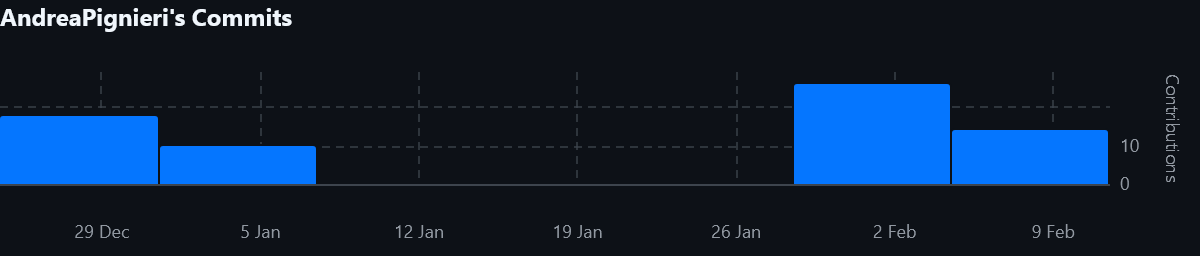
\includegraphics[width=\textwidth]{pics/AndreaPignieri's Commits.png}
    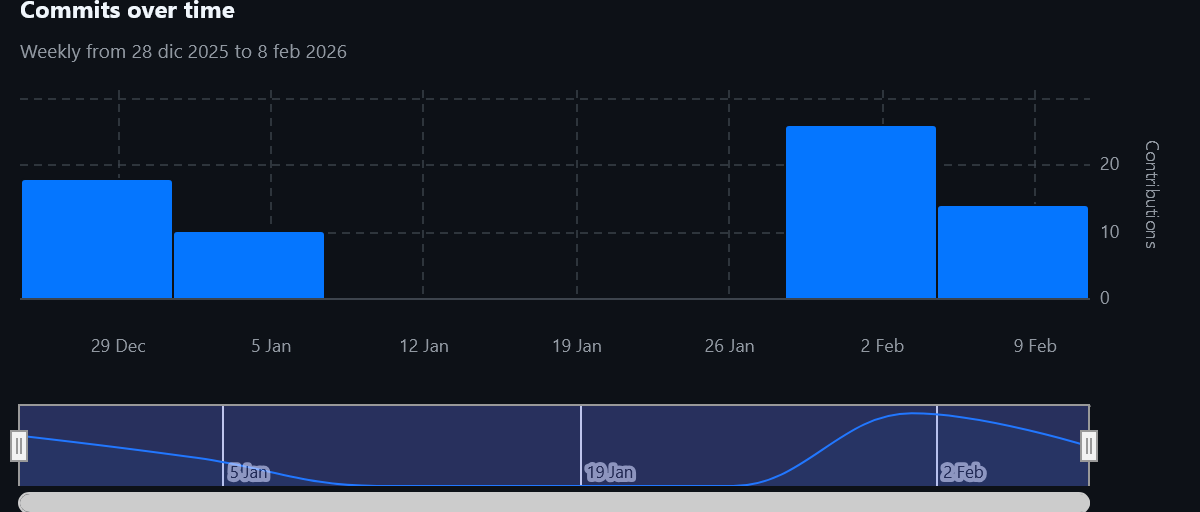
\includegraphics[width=\textwidth]{pics/Commits over time.png}
    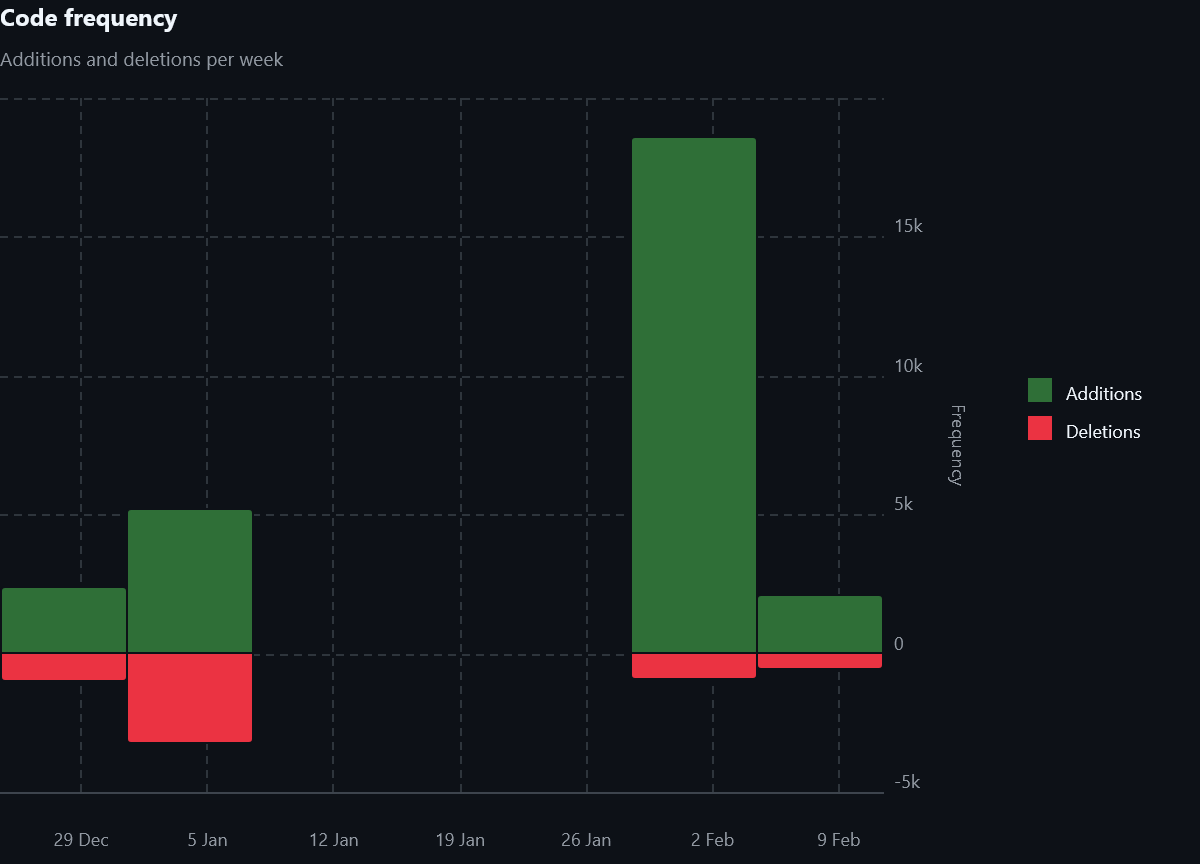
\includegraphics[width=\textwidth]{pics/Code frequency.png}
    \caption{Statistiche del repository GitHub}
\end{figure}

\section{Analisi della qualità del codice}

Per garantire la qualità e la manutenibilità del codice back-end, il progetto utilizza \textbf{SonarQube}, una piattaforma di analisi statica del codice che valuta:

\begin{itemize}[nosep]
  \item \textbf{Code smells}: problemi di design e architettura che possono compromettere la manutenibilità;
  \item \textbf{Bug}: errori potenziali che potrebbero causare comportamenti inattesi;
  \item \textbf{Vulnerabilità di sicurezza}: problemi di sicurezza che potrebbero essere sfruttati da attaccanti;
  \item \textbf{Coverage}: percentuale di codice coperta da test unitari;
  \item \textbf{Duplicazione}: presenza di codice duplicato che può essere refactorizzato;
  \item \textbf{Debito tecnico}: tempo stimato necessario per risolvere tutti i problemi rilevati.
\end{itemize}

\subsection{Report SonarQube}

L'analisi SonarQube sul codice back-end Spring Boot evidenzia:

\begin{itemize}[nosep]
  \item un livello di qualità complessivo conforme agli standard del progetto;
  \item presenza di test unitari con copertura adeguata per i componenti critici (service layer, controller principali);
  \item assenza di vulnerabilità critiche o ad alto rischio.
\end{itemize}

Il report fornisce metriche dettagliate per ogni componente (classi, metodi, linee di codice) e suggerimenti specifici per il miglioramento continuo della qualità del codice.

\begin{figure}[H]
    \centering
    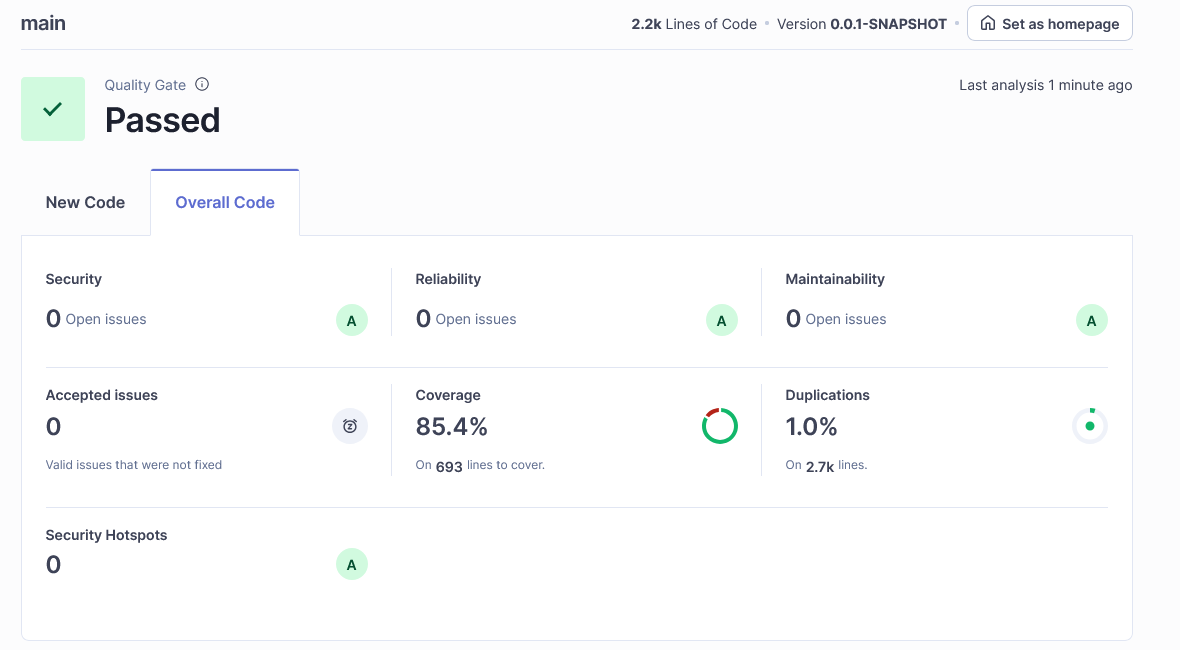
\includegraphics[width=\textwidth]{pics/SonarQubeReport.png}
    \caption{Report di qualità del codice SonarQube}
\end{figure}


\chapter{Testing e valutazione dell’usabilità}

\section{Strategia di unit testing}

Il back-end utilizza \textbf{JUnit 5} come framework di testing e \textbf{Mockito} per il mocking delle dipendenze. La strategia adottata segue il pattern \emph{Arrange-Act-Assert} (AAA) e si basa su:

\begin{itemize}[nosep]
  \item \textbf{Isolamento delle unità}: ogni test isola la classe sotto test (Service) mockando le dipendenze esterne (Repository, altri Service, componenti infrastrutturali).
  \item \textbf{Test delle responsabilità}: ogni test verifica un singolo comportamento o scenario, garantendo che i test siano focalizzati e facilmente debuggabili.
  \item \textbf{Copertura di casi positivi e negativi}: per ogni metodo critico vengono testati sia il percorso di successo che i percorsi di errore (eccezioni attese).
\end{itemize}

\subsection{Classi di equivalenza e criteri di copertura}

Per la progettazione dei test vengono identificate \textbf{classi di equivalenza} sui parametri di ingresso di ciascun metodo. Una classe di equivalenza raggruppa valori di input che producono lo stesso comportamento atteso del sistema. I test vengono progettati per coprire almeno un rappresentante per ogni classe valida e invalida.

\subsubsection*{Criteri di copertura strutturale}

I test mirano a raggiungere:

\begin{itemize}[nosep]
  \item \textbf{Copertura delle istruzioni}: ogni istruzione del codice viene eseguita almeno una volta.
  \item \textbf{Copertura dei branch}: ogni ramo condizionale (if/else, switch) viene percorso sia nel caso \texttt{true} che \texttt{false}.
  \item \textbf{Copertura dei path}: per metodi complessi con più condizioni annidate, vengono testate combinazioni significative di percorsi di esecuzione.
\end{itemize}

\subsection{Esempi di metodi testati con classi di equivalenza}

\subsubsection*{\texttt{searchProperties(criteria, page, limit)} in \texttt{PropertyService}}

Questo metodo implementa la ricerca avanzata con filtri multipli e supporto per ricerca geografica. Le classi di equivalenza identificate sono:

\begin{table}[H]
\centering
\small
\renewcommand{\arraystretch}{1.3}
\begin{tabularx}{\textwidth}{|l|X|}
\toprule
\textbf{Parametro} & \textbf{Classi di equivalenza} \\
\midrule
\texttt{criteria} & 
\begin{itemize}[nosep, leftmargin=*]
  \item \textbf{CE1}: criteri vuoti/null (ricerca senza filtri)
  \item \textbf{CE2}: criteri con filtri testuali (città, tipo, classe energetica)
  \item \textbf{CE3}: criteri con filtri numerici validi (prezzo, stanze, metratura, piano, bagni)
  \item \textbf{CE4}: criteri con filtri geografici (latitudine, longitudine, raggio)
  \item \textbf{CE5}: combinazione di filtri multipli (testuali + numerici + geografici)
  \item \textbf{CE6}: filtri numerici incoerenti (minPrice > maxPrice, minSize > maxSize) -- \emph{classe invalida}
\end{itemize} \\
\midrule
\texttt{page} & 
\begin{itemize}[nosep, leftmargin=*]
  \item \textbf{CE7}: valore valido (\(\geq 0\))
  \item \textbf{CE8}: valore negativo -- \emph{classe invalida}
\end{itemize} \\
\midrule
\texttt{limit} & 
\begin{itemize}[nosep, leftmargin=*]
  \item \textbf{CE9}: valore valido (\(> 0\))
  \item \textbf{CE10}: valore \(\leq 0\) -- \emph{classe invalida}
\end{itemize} \\
\bottomrule
\end{tabularx}
\caption{Classi di equivalenza per \texttt{searchProperties}}
\end{table}

\textbf{Casi di test implementati:}

\begin{itemize}[nosep]
  \item \texttt{searchProperties\_AllFilters\_CallsRepo}: verifica il percorso con tutti i filtri popolati (CE5), assicurando che la \texttt{Specification} venga costruita correttamente e che il repository venga chiamato con i parametri attesi.
  \item \texttt{searchProperties\_GeoFilter\_CallsRepo}: verifica il percorso con filtri geografici (CE4), testando la costruzione della query PostGIS per il calcolo della distanza.
\end{itemize}

\textbf{Copertura strutturale}: i test coprono i branch principali della costruzione della \texttt{Specification} (presenza/assenza di ciascun filtro) e verificano che i predicati vengano combinati correttamente tramite \texttt{and()}.

\subsubsection*{\texttt{createProperty(request, agentEmail)} in \texttt{PropertyService}}

Metodo critico per la creazione di immobili. Le classi di equivalenza sono:

\begin{table}[H]
\centering
\small
\renewcommand{\arraystretch}{1.3}
\begin{tabularx}{\textwidth}{|l|X|}
\toprule
\textbf{Parametro} & \textbf{Classi di equivalenza} \\
\midrule
\texttt{request.type} & 
\begin{itemize}[nosep, leftmargin=*]
  \item \textbf{CE1}: valore valido (\texttt{"SALE"}, \texttt{"RENT"})
  \item \textbf{CE2}: valore invalido (\texttt{"INVALID\_TYPE"}) -- \emph{classe invalida}
\end{itemize} \\
\midrule
\texttt{agentEmail} & 
\begin{itemize}[nosep, leftmargin=*]
  \item \textbf{CE3}: email esistente nel repository
  \item \textbf{CE4}: email non esistente -- \emph{classe invalida}
  \item \textbf{CE5}: agente esistente ma senza agenzia associata -- \emph{classe invalida}
\end{itemize} \\
\midrule
\texttt{request.amenities} & 
\begin{itemize}[nosep, leftmargin=*]
  \item \textbf{CE6}: lista vuota/null
  \item \textbf{CE7}: lista con amenity esistenti nel repository
  \item \textbf{CE8}: lista con amenity non esistenti -- \emph{classe invalida} (gestita a runtime)
\end{itemize} \\
\midrule
\texttt{request.photos} & 
\begin{itemize}[nosep, leftmargin=*]
  \item \textbf{CE9}: lista vuota/null
  \item \textbf{CE10}: lista con URL validi
\end{itemize} \\
\bottomrule
\end{tabularx}
\caption{Classi di equivalenza per \texttt{createProperty}}
\end{table}

\textbf{Casi di test implementati:}

\begin{itemize}[nosep]
  \item \texttt{createProperty\_ValidData\_SavesProperty}: verifica il percorso di successo (CE1, CE3, CE7, CE10), controllando che l'entità venga salvata con tutti i campi mappati correttamente e che le relazioni con \texttt{Amenity} e \texttt{Agency} siano stabilite.
  \item \texttt{createProperty\_InvalidType\_ThrowsException}: verifica che venga sollevata un'eccezione per tipo invalido (CE2).
  \item \texttt{createProperty\_AgentNotFound\_ThrowsException}: verifica l'eccezione per agente non trovato (CE4).
  \item \texttt{createProperty\_AgentNoAgency\_ThrowsException}: verifica l'eccezione per agente senza agenzia (CE5).
\end{itemize}

\textbf{Copertura strutturale}: i test coprono tutti i branch condizionali del metodo (controllo esistenza agente, controllo presenza agenzia, validazione tipo, gestione amenities e foto).

\subsubsection*{\texttt{register(RegisterRequest request)} in \texttt{AuthService}}

Metodo per la registrazione di nuovi utenti. Le classi di equivalenza sono:

\begin{table}[H]
\centering
\small
\renewcommand{\arraystretch}{1.3}
\begin{tabularx}{\textwidth}{|l|X|}
\toprule
\textbf{Parametro} & \textbf{Classi di equivalenza} \\
\midrule
\texttt{request.email} & 
\begin{itemize}[nosep, leftmargin=*]
  \item \textbf{CE1}: email non esistente nel repository (nuova registrazione)
  \item \textbf{CE2}: email già esistente -- \emph{classe invalida}
\end{itemize} \\
\midrule
\texttt{request.password} & 
\begin{itemize}[nosep, leftmargin=*]
  \item \textbf{CE3}: password valida (non vuota, lunghezza minima rispettata)
  \item \textbf{CE4}: password invalida (vuota, troppo corta) -- \emph{classe invalida} (validata a livello di DTO/Controller)
\end{itemize} \\
\midrule
\texttt{request.firstName, request.lastName} & 
\begin{itemize}[nosep, leftmargin=*]
  \item \textbf{CE5}: valori non nulli e non vuoti
  \item \textbf{CE6}: valori nulli o vuoti -- \emph{classe invalida} (validata a livello di DTO)
\end{itemize} \\
\bottomrule
\end{tabularx}
\caption{Classi di equivalenza per \texttt{register}}
\end{table}

\textbf{Casi di test implementati:}

\begin{itemize}[nosep]
  \item \texttt{register\_NewEmail\_SavesUser}: verifica il percorso di successo (CE1, CE3, CE5), controllando che l'utente venga salvato con password codificata e ruolo \texttt{USER} assegnato.
  \item \texttt{register\_ExistingEmail\_ThrowsException}: verifica che venga sollevata un'eccezione con messaggio appropriato per email già registrata (CE2).
\end{itemize}

\textbf{Copertura strutturale}: i test coprono il branch principale (controllo esistenza email) e verificano lo stato indotto sul repository (salvataggio con attributi corretti).

\subsubsection*{\texttt{login(LoginRequest request)} in \texttt{AuthService}}

Metodo per l'autenticazione degli utenti. Le classi di equivalenza sono:

\begin{table}[H]
\centering
\small
\renewcommand{\arraystretch}{1.3}
\begin{tabularx}{\textwidth}{|l|X|}
\toprule
\textbf{Parametro} & \textbf{Classi di equivalenza} \\
\midrule
\texttt{request.email, request.password} & 
\begin{itemize}[nosep, leftmargin=*]
  \item \textbf{CE1}: credenziali corrette (email esistente, password corrispondente)
  \item \textbf{CE2}: credenziali errate (password non corrispondente) -- \emph{classe invalida}
  \item \textbf{CE3}: utente non esistente (email non presente nel repository) -- \emph{classe invalida}
\end{itemize} \\
\bottomrule
\end{tabularx}
\caption{Classi di equivalenza per \texttt{login}}
\end{table}

\textbf{Casi di test implementati:}

\begin{itemize}[nosep]
  \item \texttt{login\_ValidCredentials\_ReturnsToken}: verifica il percorso di successo (CE1), controllando che venga generato un JWT valido e che la risposta contenga i dati utente corretti.
  \item \texttt{login\_InvalidCredentials\_ThrowsException}: verifica che venga sollevata \texttt{BadCredentialsException} per password errata (CE2).
  \item \texttt{login\_UserNotFound\_ThrowsException}: verifica l'eccezione per utente non trovato (CE3).
\end{itemize}

\textbf{Copertura strutturale}: i test coprono tutti i branch del metodo (autenticazione riuscita, fallita per credenziali errate, fallita per utente inesistente).

\subsubsection*{\texttt{createAgent(request)} in \texttt{AgentService}}

Metodo per la creazione di agenti da parte del manager di agenzia. Le classi di equivalenza sono:

\begin{itemize}[nosep]
  \item \textbf{CE1}: manager autenticato esistente con agenzia associata (caso valido).
  \item \textbf{CE2}: manager non trovato nel repository -- \emph{classe invalida}.
  \item \textbf{CE3}: manager esistente ma senza agenzia associata -- \emph{classe invalida}.
\end{itemize}

\textbf{Casi di test implementati:}

\begin{itemize}[nosep]
  \item \texttt{createAgent\_ValidRequest\_SavesAgent}: verifica il percorso di successo (CE1), controllando che l'agente venga salvato con agenzia corretta e ruolo \texttt{AGENT}.
  \item \texttt{createAgent\_ManagerNotFound\_ThrowsException}: verifica l'eccezione per manager non trovato (CE2).
  \item \texttt{createAgent\_ManagerHasNoAgency\_ThrowsException}: verifica l'eccezione per manager senza agenzia (CE3).
\end{itemize}

\subsection{Verifica dei risultati e dello stato}

Per ciascun test vengono verificati:

\begin{itemize}[nosep]
  \item \textbf{Valori di ritorno}: il metodo restituisce il valore atteso (DTO, entità, o void con effetti collaterali verificati).
  \item \textbf{Stato indotto sul repository}: tramite \texttt{verify()} di Mockito si controlla che i metodi del repository vengano chiamati con i parametri corretti e il numero di volte atteso.
  \item \textbf{Eccezioni attese}: per i casi negativi, si verifica che venga sollevata l'eccezione corretta con \texttt{assertThrows()} e, quando rilevante, che il messaggio di errore sia appropriato.
\end{itemize}

\subsection{Copertura del codice}

La copertura del codice viene misurata tramite \textbf{JaCoCo} durante l'esecuzione dei test Maven. L'obiettivo è raggiungere una copertura superiore all'80\% per le classi di servizio critiche (\texttt{PropertyService}, \texttt{AuthService}, \texttt{AgentService}) e per i componenti di sicurezza (\texttt{JwtService}, \texttt{JwtAuthenticationFilter}).

\section{Testing di integrazione e API}

I test di integrazione verificano il comportamento end-to-end delle API REST, testando l'interazione tra Controller, Service e Repository (o mock del repository, a seconda del livello di isolamento desiderato).

\subsection{Test dei Controller}

I test dei controller utilizzano \textbf{Spring Test} con \texttt{@WebMvcTest} per caricare solo il contesto web necessario, mockando i Service layer tramite \texttt{@MockBean}. Questo approccio:

\begin{itemize}[nosep]
  \item isola il layer di presentazione dal layer di business;
  \item permette di testare il mapping HTTP (URI, metodi, parametri di query, body delle richieste);
  \item verifica la serializzazione/deserializzazione JSON dei DTO;
  \item valida l'applicazione dei filtri di sicurezza e la gestione delle eccezioni a livello di controller.
\end{itemize}

\subsubsection*{Esempi di test implementati}

\begin{itemize}[nosep]
  \item \textbf{\texttt{PropertyControllerTest.shouldSearchProperties}}: verifica che l'endpoint \texttt{GET /properties} con parametri di query venga mappato correttamente, che il Service venga chiamato con i criteri corretti e che la risposta HTTP 200 contenga il JSON atteso.
  \item \textbf{\texttt{AuthControllerTest.shouldRegisterUserSuccessfully}}: verifica che \texttt{POST /auth/register} con body valido restituisca HTTP 201.
  \item \textbf{\texttt{AuthControllerTest.shouldReturnBadRequestOnInvalidRegister}}: verifica la validazione a livello di controller (HTTP 400 per dati invalidi).
  \item \textbf{\texttt{AuthControllerTest.shouldReturnConflictIfEmailExists}}: verifica la gestione delle eccezioni di business (HTTP 409 per email già esistente).
  \item \textbf{\texttt{AuthControllerTest.shouldLoginSuccessfully}}: verifica il percorso di successo del login (HTTP 200 con token JWT).
  \item \textbf{\texttt{AuthControllerTest.shouldReturnNotFoundIfUserNotFound}}: verifica la gestione di utente non trovato (HTTP 404).
\end{itemize}
\pagebreak

\subsection{Criteri di copertura per i test di integrazione}

I test di integrazione coprono:

\begin{itemize}[nosep]
  \item \textbf{Mapping degli endpoint}: correttezza dell'URI, del metodo HTTP (GET, POST, PUT, DELETE) e dei parametri (path variables, query parameters, request body).
  \item \textbf{Codici di stato HTTP}: verifica dei codici attesi (200, 201, 400, 401, 404, 409, 500) per ogni scenario.
  \item \textbf{Struttura delle response}: validazione della struttura JSON delle risposte tramite \texttt{jsonPath()} di Spring Test.
  \item \textbf{Sicurezza}: verifica che gli endpoint protetti richiedano autenticazione e che gli endpoint pubblici siano accessibili senza token.
  \item \textbf{Gestione degli errori}: verifica che le eccezioni vengano trasformate correttamente in risposte HTTP con codici e messaggi appropriati tramite \texttt{GlobalExceptionHandler}.
\end{itemize}

\subsection{Test di integrazione con database}

Per i test che richiedono un database reale (ad esempio, test end-to-end completi), viene utilizzato un database H2 in-memory configurato tramite \texttt{@SpringBootTest} con profilo di test. Questi test verificano:

\begin{itemize}[nosep]
  \item la persistenza corretta delle entità;
  \item l'integrità referenziale;
  \item le query complesse (es. ricerca geografica con PostGIS).
\end{itemize}

Tuttavia, per la maggior parte dei test di integrazione, si preferisce mockare il repository per mantenere i test veloci e isolati.

\pagebreak

\section{Valutazione dell’usabilità}

La valutazione dell’usabilità di DietiEstates25 è stata svolta tramite due approcci complementari:
(i) ispezione esperta basata sulle 10 euristiche di Nielsen, per identificare problemi sistematici dell’interfaccia;
(ii) sessioni di user testing strutturate su task rappresentativi, con raccolta di metriche quantitative e feedback qualitativo.

\subsection{Expert reviews / inspections (Nielsen Heuristics)}

\paragraph{Metodo} Heuristic Evaluation basata sulle \textbf{10 Usability Heuristics di Nielsen}.
\paragraph{Valutatori} 3 valutatori indipendenti (ispezione interna) su una build stabile.
\paragraph{Output} Lista consolidata di issue e raccomandazioni, con priorità (alta/media/bassa).

\subsubsection*{Risultati principali (sintesi consolidata)}

\begin{itemize}[nosep]
  \item \textbf{H1 -- Visibilità dello stato del sistema:} feedback positivi su caricamenti e stati di salvataggio degli annunci.
  \item \textbf{H2 -- Corrispondenza con il mondo reale:} terminologia di dominio coerente (Mq, Classe Energetica, Rating).
  \item \textbf{H3 -- Controllo e libertà dell’utente:} presente il reset dei filtri e la possibilità di annullare l'inserimento di un annuncio prima della pubblicazione.
  \item \textbf{H4 -- Coerenza e standard:} componenti UI consistenti; le icone per le recensioni e i form di inserimento seguono pattern attesi.
  \item \textbf{H7 -- Flessibilità ed efficienza:} il sistema è intuitivo per i nuovi utenti, ma la ricerca avanzata richiede un attimo prima di essere compresa.
  \item \textbf{H9 -- Recupero dagli errori:} messaggi di validazione nei form (prezzo mancante, formato email errato) potrebbero essere migliorati.
\end{itemize}

\subsection{Esperimento con utenti}

\subsubsection*{Obiettivo}

Valutare l'efficacia e la soddisfazione durante la gestione attiva dei contenuti (creazione e valutazione) oltre alla semplice consultazione:
\begin{itemize}[nosep]
  \item ricerca avanzata e filtraggio immobili;
  \item inserimento di nuovi annunci nel database (lato venditore/agente);
  \item valutazione dell'operato degli agenti tramite il sistema di recensioni.
\end{itemize}

\subsubsection*{Partecipanti}

\begin{itemize}[nosep]
  \item \textbf{Campione:} N=5 utenti (potenziali venditori/acquirenti).
  \item \textbf{Età:} 24--45 anni.
  \item \textbf{Profilo:} competenze digitali eterogenee; familiarità generica con portali immobiliari.
\end{itemize}

\subsubsection*{Task}

\begin{itemize}[nosep]
  \item \textbf{Task 1 (Search \& Filter):} trovare un immobile a Napoli con 4 stanze, circa 80 m\textsuperscript{2} e prezzo nell’intorno di 200.000€.
  \item \textbf{Task 2 (Details):} dal primo risultato, individuare \emph{classe energetica} e verificare la presenza di \emph{garage}.
  \item \textbf{Task 3 (Create Property):} creare un nuovo annuncio immobiliare inserendo dati tecnici, descrizione e prezzo, completando la pubblicazione.
  \item \textbf{Task 4 (Agent Review):} individuare il profilo di un agente e pubblicare una recensione con feedback testuale e valutazione numerica.
\end{itemize}

\subsection{Risultati}

\subsubsection*{Sintesi quantitativa}

Tutti gli utenti hanno completato con successo i task assegnati senza richiedere l'intervento del moderatore.

\begin{table}[H]
\centering
\renewcommand{\arraystretch}{1.2}
\begin{tabular}{lccccc}
\toprule
\textbf{Metrica} & \textbf{Task 1} & \textbf{Task 2} & \textbf{Task 3} & \textbf{Task 4} & \textbf{Overall} \\
\midrule
Success Rate & 100\% & 100\% & 100\% & 100\% & 100\% \\
\bottomrule
\end{tabular}
\caption{Sintesi quantitativa dell'efficacia per task}
\end{table}
\paragraph{SUS} Il punteggio SUS medio è pari a \textbf{88/100}, indicativo di una usabilità \emph{eccellente}. Nonostante tutti i partecipanti abbiano completato i task con successo, sono emersi margini di miglioramento relativi alla comunicazione del sistema verso l'utente.

\subsubsection*{Sintesi qualitativa}

\paragraph{Punti di forza osservati}
\begin{itemize}[nosep]
  \item \textbf{Workflow di creazione fluido}: il form di inserimento immobile è stato percepito come ben strutturato, evitando il senso di sopraffazione nonostante la mole di dati richiesti.
  \item \textbf{Sistema di recensioni immediato}: l'interfaccia di rating e commento è risultata familiare, rapida e priva di attriti cognitivi.
  \item \textbf{Efficacia dei risultati}: la precisione dei parametri di ricerca permette di individuare l'immobile desiderato con pochissimi passaggi.
\end{itemize}

\paragraph{Criticità ricorrenti}
\begin{itemize}[nosep]
  \item \textbf{Chiarezza dei messaggi di errore}: in alcuni casi di validazione fallita (es. formati dati specifici), i messaggi restituiti dal sistema sono stati percepiti come troppo tecnici o non sufficientemente esplicativi sulla risoluzione del problema.
  \item \textbf{Densità visiva della ricerca}: la sezione dei filtri avanzati, pur essendo completa, presenta una densità di controlli che può inizialmente disorientare l'utente meno esperto.
  \item \textbf{Feedback di conferma}: dopo la pubblicazione di un annuncio o l'invio di una recensione, gli utenti hanno suggerito la necessità di un feedback visivo più marcato (es. una modale di successo o un redirect esplicito) per confermare l'avvenuta operazione.
\end{itemize}

\pagebreak

\subsection{Conclusioni e raccomandazioni}

In base ai risultati del testing e all'analisi delle euristiche, le priorità di miglioramento individuate sono:

\begin{itemize}[nosep]
  \item \textbf{Alta}: \textbf{Refactoring della messaggistica di errore}. Tradurre i codici di errore del back-end in suggerimenti testuali "user-friendly" che indichino chiaramente come correggere i dati inseriti.
  \item \textbf{Media}: \textbf{Ottimizzazione UI dei filtri}. Riorganizzare il layout della ricerca avanzata (es. tramite sezioni collassabili) per ridurre il carico cognitivo iniziale.
  \item \textbf{Bassa}: \textbf{Potenziamento dei feedback visivi}. Introdurre notifiche "toast" o modali di conferma più evidenti al completamento dei flussi principali (creazione immobile, invio recensione, modifica profilo).
\end{itemize}
\end{document}